\chapter{结构动响应数值算法}
对于结构动力学问题,在经过合适的空间离散离散离散之后,得到一个关于时间的二阶常微分方程,即结构动力学运动方程(\ref{eq:DyEq})
\begin{equation}
	M\ddot{U}(t)+C\dot{U}(t)+KU(t)=F(t)\label{eq:DyEq}
\end{equation}
带有初值条件(\ref{eq:DyEqInitCon})
\begin{equation}
{U}(0)={^0\!U}\qquad \dot{U}(0)={^0\!\dot{U}}\label{eq:DyEqInitCon}
\end{equation}

对于该微分方程的求解,最常用的技术手段就是直接积分法,该方法的要求运动方程(\ref{eq:DyEq})在离散的时刻精确满足。同时假定位移和速度的更新方程,利用离散时刻的平衡方程求得对应时刻的加速度,进而求得速度和位移。特别地,自从Newmark-$\beta$算法\cite{Newmark1959}、Wilson-$\theta$法\cite{Wilson1968}和Houbolt法\cite{Chopra2011}等直接积分法提出以来,许多的研究学者在此之后基于各种原理提出了许多性能优良的积分算法。各种不同类型的直接积分法可以参见书籍\cite{Wood,book:dover,Zienkiewicz1991a,Hairer1993,ErnstHairer1996}以及两篇关于显、隐式直接积分法的综述文章\cite{Dokainish1989,Subbaraj1989}。

在方程(\ref{eq:DyEq})中的$M,C,K$分别表示质量、阻尼和刚度矩阵;而$F(t)$表示系统所受到外力荷载,它一般情况下是关于时间$t$的已知函数;而$U(t)$表示系统的位移向量,而其上标的$(\cdot{})$代表对时间的微分,亦即$\dot{U}(t),\ddot{U}(t)$分别表示其速度和加速度。

特别地,若引入中间变量$\dot{U}(t)=V(t)$可将二阶的微分方程(\ref{eq:DyEq})转换为一阶微分方程组
\begin{equation}
\begin{bmatrix}
\dot{U}(t)\\
\dot{V}(t)
\end{bmatrix}=\begin{bmatrix}
\mathbf{0}&\mathbf{I}\\
-M^{-1}K&-M^{-1}C
\end{bmatrix}\begin{bmatrix}
{U}(t)\\
{V}(t)
\end{bmatrix}+\begin{bmatrix}
\mathbf{0}\\
M^{-1}F(t)
\end{bmatrix}\label{eq:DynqFirstOrder}
\end{equation}
其初始条件为
\begin{equation}
{U}(0)={^0\!U}\qquad V(0)={^0\!\dot{U}}
\end{equation}
其中,$\mathbf{0}$和$\mathbf{I}$分别为零矩阵和单位矩阵\footnote{其矩阵维度与系统自由度数相同。特别地,在不引起混淆的情况下,后面都不再特别指明矩阵的维度问题。}。于是,在常微分方程理论中的数值算法都可以运用到该一阶微分方程中求解。但是在转换后的位移-速度场情况下进行求解,系数矩阵的维度增加,同时位移、速度的微分关系只能以弱形式满足。需要说明的是,在后文中提及算法设计时所说的位移-速度场亦指该算法的设计是以一阶运动方程(\ref{eq:DynqFirstOrder})为基础的;而(单)位移场则说明算法设计是以二阶运动方程(\ref{eq:DyEq})为基础的。

一般情况下,对多自由度运动方程进行算法的设计和分析是一件非常繁琐和复杂的工作。幸运的是,借助模态正交性原则\cite{book:dover}且假设阻尼为经典的粘性阻尼,可以将多自由度运动方程(\ref{eq:DyEq})解耦为单自由度模态方程
\begin{equation}
\ddot{u}(t)+2\xi\omega\dot{u}(t)+\omega^2u(t)=f(t)
\end{equation}
其中,$\xi,\omega$和$f(t)$分别为阻尼率、系统的固有频率和模态外激励力;$u(t)$为未知的位移。

类似的,对于一阶解耦的运动方程也可以由上述一阶位移场的运动方程经引入中间变量转换得到。这里给出另外一种等价表述方式\cite{Fung1996e,Fung1996a}
\begin{equation}
\left\{
\begin{aligned}
\dot{y}_1(t)&=\lambda_2y_1(t)+f(t)\\
\dot{y}_2(t)&=\lambda_1y_2(t)+f(t)
\end{aligned}\right.
\end{equation}
其中,
\begin{equation}
\lambda_{1,2}=-\xi\omega\pm j\sqrt{1-\xi^2}\omega
\end{equation}
而$j=\sqrt{-1}$为虚数单位且$0\le\xi<1$。原始的一阶微分方程的解$u(t)$与该一阶方程组的解$y_1(t),y_2(t)$的关系为
\begin{equation}
\left\{
\begin{aligned}
y_1(t)&=\dot{u}(t)-\lambda_1u(t)\\
y_2(t)&=\dot{u}(t)-\lambda_2u(t)
\end{aligned}
\right.
\end{equation}
于是就有
\begin{equation}
u(t)=-\frac{y_1(t)-y_2(t)}{\lambda_1-\lambda_2}
\end{equation}
注意,变量$\lambda_{1,2}$和$y_{1,2}(t)$为复数。而最终的计算结果$u(t)$为实数。

迄今为止,构造直接积分算法的主要框架有
\begin{itemize}
\item[$\bigstar$] 有限差分法(线性多步法)[Finite Difference Methods/Linear Multistep Methods]。
\item[$\bigstar$] 多级法(Runge-Kutta法)[Multistage Methods/Runge-Kutta Methods]。
\item[$\bigstar$] 加权残值法[Weighted Residual Methods]。
\item[$\bigstar$] 泰勒级数配点法[Taylor Series Collocation Methods]。
\item[$\bigstar$] 哈密顿原理/定律[Hamilton's Principle/Law]。
\item[$\bigstar$] 最小二乘法[Least-Squares Methods]。
\item[$\bigstar$] 时间子步策略[Composite Sub-steps Techinques]。
\item[$\bigstar$] 结构依赖型参数策略[Structure-dependent Parameters Techinques]。
\end{itemize}

本章后续内容,将对这些不同的策略和框架算法进行简单的总结和归纳。同时,在作者力所能及的范围内尽可能阐述清楚。
% ========================================================================
\section{有限差分法(线性多步法)}
考虑带有初值条件$y(0)=y(t_0=0)$的单变量一阶微分方程
\begin{equation}
\dot{y}(t)=f(y,t)\label{eq:firstSystem}
\end{equation}
在时间$t\in[0,T]$上的数值解。将时间区间$[0,T]$划分为互不重叠的相等的小区间,即
\begin{equation}
[0,T]=\bigcup_{n=0}^{N-1}[t_n,t_{n+1}]
\end{equation}
而$\Delta t=t_{n+1}-t_n$为时间步长大小,在本文中都假定为常值不可变,亦即本文将不考虑变时间步长的积分算法。而时间积分算法一般是假定在$t_n$时刻之前的响应已知,求$t_{n+1}$时刻的响应。

针对一阶微分方程(\ref{eq:firstSystem})的$k$-步线性多步法\cite{book:dover,Gear1971a}被定义如下
\begin{equation}
\begin{split}
\alpha_0{^{t+\Delta t}\!y}+&\alpha_1{^{t}\!y}+\cdots+\alpha_k{^{t+(1-k)\Delta t}\!y}\\
&=\Delta t[\beta_0f({^{t+\Delta t}\!y},t_{n+1}+\beta_1f({^{t}\!y},t_{n})+\cdots+\beta_kf({^{t+(1-k)\Delta t}\!y},t_{n+1-k})]
\end{split}
\end{equation}
其中,$\alpha_i,\beta_i$为算法参数。上述方程可以改成为
\begin{equation}
\sum_{i=0}^k\{\alpha_i{^{t+(1-i)\Delta t}\!y}+\Delta t\beta_if({^{t+(1-i)\Delta t}\!y},t_{n+1-i}) \}=0\label{eq:firstsystemLMS}
\end{equation}
注意到各项之间是线性关系,且当$\beta_0=0$时,该线性$k$-步法为显式格式;否则为$k$-步隐式算法。

考虑到在求解结构动力学问题时,经过有限元离散之后往往等到一个二阶微分方程,故针对一般形式的二阶微分方程
\begin{equation}
\ddot{y}=f(\dot{y}(t),y(t),t)=g_0y(t)+g_1\dot{y}(t)+h(t)\label{eq:secondsystem}
\end{equation}
其中,$g_0,g_1\in\mathbf{R}$是常数。同时该微分方程也是假定为线性的。对于二阶微分方程(\ref{eq:secondsystem})的$k$-步的线性多步法\cite{Geradin2006}
\begin{equation}
\sum_{i=0}^{k}\{\alpha_i{^{t+(1-i)\Delta t}\!y}+\Delta t\beta_ig_1{^{t+(1-i)\Delta t}\!y}+\Delta t^2\gamma_i[g_0{^{t+(1-i)\Delta t}\!y}+h(t_{n+1-i})]\}=0
\end{equation}
其中,$\alpha_i,\beta_i$和$\gamma_i$均为算法参数。当参数$\beta_0=0$,上述算法得到显式算法;否则是隐式的。关于该公式的更多的应用可以参考原文\inlinecite{Geradin2006}。
%===================================================================
\subsection{向前欧拉法}
向前欧拉法可以通过将$y(t_{n+1})={^{n+1}\!y}$在$t_n$时刻进行泰勒级数展开获得。即
\begin{equation}
{^{n+1}\!y}={^{n}\!y}+\Delta t{^n\!\dot{y}}+\frac{\Delta t^2}{2!}{^n\!\ddot{y}}+\frac{\Delta t^3}{3!}{^n\!y^{(3)}}+\cdots
\end{equation}
上式可以写为
\begin{equation}
{^{n+1}\!y}={^{n}\!y}+\Delta t{^n\!\dot{y}}+\mathcal{O}(\Delta t^2)
\end{equation}
其中,$\mathcal{O}(\Delta t^2)$表示为局部截断误差。因此一阶导数可以由下列的向前差分得到
\begin{equation}
{^n\!\dot{y}}=\frac{{^{n+1}\!y}-{^n\!y}}{\Delta t}+E_{trunc}(y,\Delta t)
\end{equation}

于是,向前欧拉法由下式给出
\begin{equation}
\frac{{^{n+1}\!y}-{^n\!y}}{\Delta t}={^n\!\dot{y}}
\end{equation}
亦即
\begin{equation}
{^{n+1}\!y}={^n\!y}+\Delta t{^n\!\dot{y}}={^n\!y}+\Delta tf({^n\!y},t_n)
\end{equation}
可以看出,当在$t_n$时刻的${^n\!y}$已知时,根据上述就可以求得在$t_{n+1}$时刻的${^{n+1}\!y}$值,而不需要求解(非)线性方程组。故向前欧拉法是单步显式方法,同时该算法是一阶条件稳定算法。

向前欧拉法是最简单也是最早被提出的一个数值算法。后续的许多学者基于此提出了许多改进欧拉法的方案,进而引出了许多其他性能较优的算法。感兴趣的读者可以参考书籍\inlinecite{Butcher2008,Jackiewicz2009}。
\subsection{向后欧拉法}
同理,若关于时间的一阶导数$\dot{y}(t)$用向后差分公式进行逼近,则可以得到向后欧拉法
\begin{equation}
{^{n+1}\!y}={^n\!y}+\Delta t{^{n+1}\!\dot{y}}={^n\!y}+\Delta tf({^{n+1}\!y},t_n)
\end{equation}
可以看出,为了求解${^{n+1}\!y}$,需要求解一个线性方程组或者非线性方程组(取决于$f(y,t)$的形式),于是向后欧拉法是单步隐式算法。同时,向后欧拉法是无条件稳定带渐进消弭特性的算法。即是L-稳定的。
\subsection{广义梯形算法}
通过将${^n\!\dot{y}}$和${^{n+1}\!\dot{y}}$进行凸组合\cite{book:dover,Wood},即$(0\le\alpha\le1)$
\begin{equation}
{^{n+\alpha}\!\dot{y}}=(1-\alpha){^n\!\dot{y}}+\alpha{^{n+1}\!\dot{y}}
\end{equation}
结合
\begin{equation}
{^{n+1}\!y}-{^n\!y}=\Delta t{^{n+\alpha}\!\dot{y}}
\end{equation}
就可以得到具有如下形式的广义梯形公式
\begin{equation}
{^{n+1}\!y}={^n\!y}+\Delta t[(1-\alpha){^n\!\dot{y}}+\alpha{^{n+1}\!\dot{y}}]
\end{equation}
需要说明的时,当$\alpha=0$时,广义梯形公式退化为向前欧拉法;当$\alpha=1$时,广义梯形公式退化为向后欧拉法;而当$\alpha=\frac12$时,得到梯形公式
\begin{equation}
{^{n+1}\!y}={^n\!y}+\frac{\Delta t}{2}({^n\!\dot{y}}+{^{n+1}\!\dot{y}})
\end{equation}
该梯形公式也称为Crank-Nicolson公式。特别地,类似于梯形公式的运用在后续算法设计中使用频率相当高,读者应引起注意。

对于如下的半离散化方程
\begin{equation}
M\dot{d}+Kd=F
\end{equation}
的广义梯形公式形式为
\begin{align}
M{^{n+1}\!\dot{d}}+K{^{n+1}\!d}&={^{n+1}\!F}\\
{^{n+1}\!d}&={^n\!d}+\Delta t{^{n+\alpha}\!\dot{d}}\\
{^{n+\alpha}\!\dot{d}}&={^n\!\dot{d}}(1-\alpha)+{^{n+1}\!\dot{d}}\alpha
\end{align}
将上述三式化为位移$d$和$F$的关系,则为
\begin{equation}
(M+\alpha\Delta tK){^{n+1}\!d}=[M-(1-\alpha)\Delta tK]{^n\!d}+\Delta t[{^{n+1}\!F}\alpha+{^n\!F}(1-\alpha)]
\end{equation}
当$\alpha=\theta$时,上述算法也称为$\theta$-格式\cite{Wood}。
\subsection{中点公式}
当考虑变量$y$的如下$\alpha$凸组合时
\begin{equation}
{^{n+\alpha}\!y}={^{n+1}\!y}\alpha+{^n\!y}(1-\alpha)
\end{equation}
同时,关于时间$t$的$\beta$凸组合有
\begin{equation}
t_{n+\beta}=\beta t_{n+1}+(1-\beta)t_n
\end{equation}
则变量$y$在区间$[t_n,t_{n+1}]$的中点值${^{n+1/2}\!y}$为
\begin{equation}
{^{n+1/2}\!y}=\frac{{^{n+1}\!y}+{^n\!y}}{2}
\end{equation}
与此同时,关于时间的中点值为
\begin{equation}
t_{n+\frac{1}{2}}=\frac{t_{n+1}+t_n}{2}
\end{equation}

对于一般的非线性情况,下式一般情况下不成立
\begin{equation}
{^{n+1/2}\!y}\neq y(t_{n+\frac{1}{2}})
\end{equation}

根据${^{n+1/2}\!y}$是否做近似处理时,可以得到两个中点公式:

\textbf{显式中点公式\cite{Gear1971a}}
\begin{align}
{^{n+1}\!y}&={^n\!y}+\Delta t{^{n+1/2}\!\dot{y}}={^n\!y}+\Delta tf({^{n+1/2}\!{y}},t_{n+\frac{1}{2}})\\
{^{n+1/2}\!{y}}&={^n\!y}+\frac{\Delta t}{2}f({^n\!y},t_n)\\
t_{n+\frac12}&=\frac{t_{n+1}+t_n}{2}
\end{align}

\textbf{隐式中点公式\cite{Hairer1993}}
\begin{align}
{^{n+1}\!y}&={^n\!y}+\Delta t{^{n+1/2}\!\dot{y}}={^n\!y}+\Delta tf({^{n+1/2}\!{y}},t_{n+\frac{1}{2}})\\
t_{n+\frac12}&=\frac{t_{n+1}+t_n}{2}
\end{align}

对于线性系统,中点公式将退化为梯形公式(Crank-Nicolson公式)。

\subsection{中心差分法}
对于一阶系统(\ref{eq:firstSystem}),使用中心差分公式计算其一阶导数项,则有其中心差分格式为
\begin{equation}
{^n\!\dot{y}}=\frac{{^{n+1}\!y}-{^{n-1}\!y}}{2\Delta t}
\end{equation}
亦即
\begin{equation}
{^{n+1}\!y}={^{n-1}\!y}+2\Delta t{^n\!\dot{y}}={^{n-1}\!y}+2\Delta tf({^n\!y},t_n)
\end{equation}

而对于二阶微分方程
\begin{equation}
\ddot{y}(t)=f(y(t),\dot{y}(t),t)\label{eq:secondSystem}
\end{equation}
其二阶导数的中心差分仍可由泰勒级数展开得到,即
\begin{equation}
{^n\!\ddot{y}}=\frac{{^{n+1}\!y}-2{^n\!y}+{^{n-1}\!y}}{\Delta t^2}
\end{equation}
于是,二阶微分方程(\ref{eq:secondSystem})的中心差分格式为
\begin{equation}
{^{n+1}\!y}=-{^{n-1}\!y}+2{^n\!y}+\Delta t^2{^n\!\ddot{y}}=-{^{n-1}\!y}+2{^n\!y}+\Delta t^2f({^n\!y},{^n\!\dot{y}},t)
\end{equation}

对于位移场的运动方程(\ref{eq:DyEq}),其中心差分格式则可描述如下
\begin{align}
M{^{t}\!\ddot{U}}+C{^{t}\!\dot{U}}+K{^{t}\!U}&={^{t}\!F}\\
{^t\!\dot{U}}&=\frac{1}{2\Delta t}({^{t+\Delta t}\!{U}}-{^{t-\Delta t}\!{U}})\\
{^t\!\ddot{U}}&=\frac{1}{\Delta t^2}({^{t+\Delta t}\!{U}}-2{^t\!{U}}+{^{t-\Delta t}\!{U}})
\end{align}

对于给定的初始条件,中心差分法并没有办法进行自启动;于是还需要引入额外的启动机制去计算${^{-\Delta t}\!U}$才能进行后续计算。常用的一个启动机制\cite{张雄2007}为
\begin{equation}
{^{-\Delta t}\!U}={^0\!U}-{^0\!\dot{U}}\Delta t+\frac{1}{2}{^0\!\ddot{U}}\Delta t^2
\end{equation}
\subsection{Houbolt算法}
Houbolt算法\cite{Geradin2006}是最早计算结构动力学数值响应的算法之一。该算法使用了在$t+\Delta t$时刻的运动平衡方程和两个向后微分公式。而向后微分公式通过使用连续四个节点的值来构造三次多项式完成。其算法格式可以描述如下
\begin{subequations}
\begin{align}
M{^{t+\Delta t}\!\ddot{U}}+C{^{t+\Delta t}\!\dot{U}}+K{^{t+\Delta t}\!U}&={^{t+\Delta t}\!F}\\
{^{t+\Delta t}\!\dot{U}}&=\frac{1}{6\Delta t}(11{^{t+\Delta t}\!U}-18{^{t}\!U}+9{^{t-\Delta t}\!U}-2{^{t-2\Delta t}\!U})\\
{^{t+\Delta t}\!\ddot{U}}&=\frac{1}{\Delta t^2}(2{^{t+\Delta t}\!U}-5{^{t}\!U}+4{^{t-\Delta t}\!U}-{^{t-2\Delta t}\!U})
\end{align}
\end{subequations}
通过使用速度和加速度的更新公式,在平衡方程中消去速度和加速度得到仅关于位移的差分方程如下
\begin{equation}
\begin{split}
\left[\frac{2}{\Delta t^2}M+\frac{11}{6\Delta t}+K\right]{^{t+\Delta t}\!U}&={^{t+\Delta t}\!F}+\left[\frac{5}{\Delta t^2}M+\frac{3}{\Delta t}C\right]{^t\!U}\\
&-\left[\frac{4}{\Delta t^2}M+\frac{3}{2\Delta t}C\right]{^{t-\Delta t}\!U}+\left[\frac{1}{\Delta t^2}M+\frac{1}{3\Delta t}C\right]{^{t-2\Delta t}\!U}
\end{split}
\end{equation}
显然,Houbolt算法不是自启动的。对于在第一个时间步长内需要知道${^{-\Delta t}\!U}$和${^{-2\Delta t}\!U}$,这就意味着需要引入额外的启动机制。同时该算法是无条件稳定的、二阶精度的隐式算法。Houbolt算法在高频段引入了很强的数值耗散。严格地说,它具有渐进消弭特性,即当$\omega\Delta t\to \infty$时,有$\rho_{\infty}=0$。它的无条件稳定性加消弭特性意味着Houbolt算法是L-稳定的。同时它的低频段耗散和相对周期误差在常用的数值算法中也是最高的,这也可以看成它除了非自启动外的另外一个重要的缺陷。

当考虑Geradin给出的对于二阶微分方程的如下逼近格式\cite{JasonHar2012}时,
\begin{subequations}
\begin{align}
M{^{t+\Delta t}\!\ddot{U}}+C{^{t+\Delta t}\!\dot{U}}+K{^{t+\Delta t}\!U}&={^{t+\Delta t}\!F}\\
\sum_{i=0}^{k}\alpha_i{^{t+(1-i)\Delta t}\!U}&=\Delta t\sum_{i=0}^{k}\beta_i{^{t+(1-i)\Delta t}\!\dot{U}}\\
\sum_{i=0}^{k}\gamma_i{^{t+(1-i)\Delta t}\!U}&=\Delta t^2\sum_{i=0}^{k}\eta_i{^{t+(1-i)\Delta t}\!\ddot{U}}
\end{align}\label{eq:SecondSystemBDF}
\end{subequations}
Houbolt算法则可以由以下参数表示:$(k=3)$
\begin{equation}
\left\{\begin{aligned}
\alpha_0&=11,\alpha_1=-18,\alpha_2=9,\alpha_3=-2\\
\beta_0&=6,\beta_1=\beta_2=\beta_3=0\\
\gamma_0&=2,\gamma_1=-5,\gamma_2=4,\gamma_3=-1\\
\eta_0&=1,\eta_1=\eta_2=\eta_3=0
\end{aligned}\right.
\end{equation}
\subsection{带终点加速度的中点公式}
当半离散化的位移场二阶运动微分方程$(\ref{eq:DyEq})$在$t_{n+\frac{1}{2}}$时,有
\begin{equation}
M{^{t+\Delta t/2}\!\ddot{U}}+C{^{t+\Delta t/2}\!\dot{U}}+K{^{t+\Delta t/2}\!U}={^{t+\Delta t/2}\!F}\label{eq:Tamma13.56}
\end{equation}
同时,其速度和位移的更新公式为
\begin{subequations}
\begin{align}
{^{t+\Delta t}\!U}&={^t\!U}+\Delta t{^{t+\Delta t/2}\!\dot{U}}\\
{^{t+\Delta t}\!\dot{U}}&={^t\!\dot{U}}+\Delta t{^{t+\Delta t/2}\!\ddot{U}}
\end{align}
\end{subequations}
在方程(\ref{eq:Tamma13.56})中的位移、速度、加速度以及外力在时刻$t_{n+\frac{1}{2}}$的逼近表达式为
\begin{equation}
\left\{\begin{split}
{^{t+\Delta t/2}\!{U}}&=\frac{1}{2}({^t}\!{U}+{^{t+\Delta t}\!{U}})\\
{^{t+\Delta t/2}\!\dot{U}}&=\frac{1}{2}({^t}\!\dot{U}+{^{t+\Delta t}\!\dot{U}})\\
{^{t+\Delta t/2}\!\ddot{U}}&=\frac{1}{2}({^t}\!\ddot{U}+{^{t+\Delta t}\!\ddot{U}})\\
{^{t+\Delta t/2}\!F}&=\frac{1}{2}({^t\!F}+{^{t+\Delta t}\!F})
\end{split}\right.\label{eq:Tamma13.58}
\end{equation}

将等式(\ref{eq:Tamma13.58})带入上两式,就可得到
\begin{equation}
\begin{split}
\left[\frac{1}{2}M+\frac{\Delta t}{4}C+\frac{\Delta t^2}{8}K\right]&{^{t+\Delta t}\!\ddot{U}}=\frac{1}{2}({^t\!F}+{^{t+\Delta t}\!F})\\
&-\left[\frac{1}{2}M+\frac{\Delta t}{4}C+\frac{\Delta t^2}{8}K\right]{^t\!\ddot{U}}-\left[C+\frac{\Delta t}{2}K\right]{^t\!\dot{U}}-K{^t\!U}
\end{split}
\end{equation}
带有位移和速度更新公式
\begin{subequations}
\begin{align}
{^{t+\Delta t}\!U}&={^t\!U}+{^t\!\dot{U}}\Delta t+\frac{\Delta t^2}{4}({^t\!\ddot{U}}+{^{t+\Delta t}\!\ddot{U}})\\
{^{t+\Delta t}\!\dot{U}}&={^t\!\dot{U}}+\frac{\Delta t}{2}({^t\!\ddot{U}}+{^{t+\Delta t}\!\ddot{U}})
\end{align}
\end{subequations}

这个算法被K. K. Tamma等人称为带终点加速度的中点公式\cite{JasonHar2012}[Midpoint Rule method with end-point acceleration](MPR-EPA)。同时在上一个时间步长内的加速度在当前的计算中起着很重要的作用。特别地,该算法对线性结构动力学系统是能量、动量以及角动量都是守恒的。

\subsection{Newmark算法}
在众多的求解结构动力学数值响应算法中,Newmark家族算法\cite{Newmark1959}可能是被公认使用最为广泛的算法。该算法在时间区间$[t_n,t_{n+1}]$内使用加速度的凸组合进行计算,即
\begin{equation}
\hat{\ddot{U}}=(1-\gamma){^t\!\ddot{U}}+\gamma{^{t+\Delta t}\!\ddot{U}}
\end{equation}
其中,$\gamma$表示自由参数。通过使用在$t_{n+1}$时刻的平衡方程,同时对上述进行积分得到下列的Newmark算法家族:
\begin{subequations}
\begin{align}
M{^{t+\Delta t}\!\ddot{U}}+C{^{t+\Delta t}\!\dot{U}}+K{^{t+\Delta t}\!U}&={^{t+\Delta t}\!F}\\
{^{t+\Delta t}\!{U}}&={^t\!U}+{^t\!\dot{U}}\Delta t+\frac{\Delta t^2}{2}[(1-2\beta){^t\!\ddot{U}}+2\beta{^{t+\Delta t}\!\ddot{U}}]\\
{^{t+\Delta t}\!\dot{U}}&={^t\!\dot{U}}+\Delta t[(1-\gamma){^t\!\ddot{U}}+\gamma{^{t+\Delta t}\!\ddot{U}}]
\end{align}\label{eq:Newmark}
\end{subequations}
其中,参数$\gamma,\beta$控制着算法的数值性能。同时Newmark算法运用十分广泛。在线性结构动力学中,使用最广泛的是a-形式。即先显式的求解位移和速度
\begin{subequations}
\begin{align}
{^{t+\Delta t}\!\widetilde{U}}&={^t\!U}+{^t\!\dot{U}}\Delta t+\frac{\Delta t^2}{2}(1-2\beta){^t\!\ddot{U}}\\
{^{t+\Delta t}\!\widetilde{\dot{U}}}&={^t\!\dot{U}}+\Delta t(1-\gamma){^t\!\ddot{U}}
\end{align}\label{eq:NewmarkUVW}
\end{subequations}
其初始加速度${^0\!\ddot{U}}$由初始时刻的平衡方程得到
\begin{equation}
{^0\!\ddot{U}}=M^{-1}({^0\!F}-C{^0\!\dot{U}}-K{^0\!U})
\end{equation}
于是,在$t_{n+1}$时刻的加速度由求解下来方程组得到
\begin{equation}
(M+\gamma \Delta tC+\beta\Delta t^2K){^{t+\Delta t}\!\ddot{U}}={^{t+\Delta t}\!F}-C{^{t+\Delta t}\!\widetilde{\dot{U}}}-K{^{t+\Delta t}\!\widetilde{U}}
\end{equation}
同时,在$t_{n+1}$时刻的速度和位移由
\begin{subequations}
\begin{align}
{^{t+\Delta t}\!{U}}&={^{t+\Delta t}\!\widetilde{U}}+\beta\Delta t^2{^{t+\Delta t}\!\ddot{U}}\\
{^{t+\Delta t}\!\dot{U}}&={^{t+\Delta t}\!\widetilde{\dot{U}}}+\gamma\Delta t{^{t+\Delta t}\!\ddot{U}}
\end{align}
\end{subequations}
计算而得。

Newmark算法的无条件稳定性的要求
\begin{equation}
2\beta\ge\gamma\ge\frac{1}{2}
\end{equation}
对于条件稳定性,应满足条件
\begin{equation}
\gamma\ge\frac{1}{2},\quad\beta<\frac{1}{2}\gamma\quad\text{和}\quad\Omega\le\Omega_{cr}
\end{equation}
其中,$\Omega=\omega\Delta t$并且
\begin{equation}
\Omega_{cr}=\frac{\xi(\gamma-\frac{1}{2})+\sqrt{\frac{1}{2}\gamma-\beta+\xi^2(\gamma-\frac12)^2}}{\frac{1}{2}\gamma-\beta}\label{eq:Tamma13.76}
\end{equation}

需要注意的是,其稳定性条件应对系统的每个模态系统均成立,故一般情况下,最高阶模态系统应满足条件(\ref{eq:Tamma13.76})。特别地,对于参数$\gamma<\frac{1}{2}$,Newmark算法将产生负阻尼,进而产生无界振动的数值解;而对于$\gamma>\frac{1}{2}$,将产生正的数值阻尼,且此时系统的粘性阻尼不能扩大系统的临界采样频率,故对于系统的模态阻尼估计不充分时,临界采样频率建议取值如下
\begin{equation}
\Omega_{cr}=\frac{1}{\sqrt{\gamma/2-\beta}}
\end{equation}
同时,当$\gamma>\frac12$,Newmark算法尽管引入了数值耗散,但是算法的精度却退化为一阶。同时对于给定的$\gamma>\frac{1}{2}$,可以通过选择$\beta$来实现最优耗散,即高频耗散最大化。其$\beta$取值为
\begin{equation}
\beta=\frac{(\gamma+\frac{1}{2})^2}{4}
\end{equation}
Newmark算法带有参数$\beta=1$和$\gamma=\frac{3}{2}$提出了可能的最大高频耗散,但该算法对低频求解精度较低,一般很少使用。

于是,大多数情况下,$\gamma=\frac{1}{2}$被使用;此时算法没有数值耗散,但实现二阶精度。

当参数$\gamma,\beta$选择不同的值时,可以产生不同的数值直接算法,如下表所示:
\begin{table}[htbp]
\bicaption[table1]{}{Newmark算法家族的著名成员}{Table$\!$}{Some well-known members for the Newmark family}
\vspace{0.5em}\centering\wuhao
\begin{tabular}{ccccc}
\toprule[1.5pt]
$\gamma$&$\beta$&名称&精度&稳定性\\
\midrule[1pt]
$1/2$ & $0$ & 中心差分法/Leap-Frog格式 & 2 & $\Omega_{cr}\le2$\\
$1/2$ & $1/12$ & Fox-Goodwin格式 & 3 & $\Omega_{cr}\le\sqrt{6}$\\
%$1/2$ & $1/10$ & Wilson-$\theta$($\theta=1.0$) & 2 & $\Omega_{cr}\le2\sqrt{3}$\\
$1/2$ & $1/6$ & 线平均加速度法 & 2 & $\Omega_{cr}\le2\sqrt{3}$\\
$1/2$ & $1/4$ & 常平均加速度法/Trapeoidal规则 & 2 & $\Omega_{cr}\le\infty$\\
$1/2$ & $1/2$ & Lee's算法\cite{Lees1966} & 2 & $--$\\
$3/2$ & $4/5$ & Galerkin方法 & 1 & $--$\\
$3/2$ & $1$ & 向后微分公式 & 1 & $--$\\
\bottomrule[1.5pt]
\end{tabular}
\end{table}

其中,中心差分法是显式的,也是被认为最为经济、求解方便的积分算法,在显式算法中使用较广;对于常平均加速度算法,该算法在二阶的隐式算法中,拥有最小的误差主项\cite{Dahlquist1963},同时该算法也是Trapeoidal规则在二阶运动方程中的体现;对于Fox-Goodwin格式,当$C\neq\mathbf{0}$时,实现三阶精度,而当无阻尼时,可以实现四阶精度。

\subsubsection{基于有限元离散的加权残差推导}
Newmark算法除了使用在$t+\Delta t$时刻的位移和速度的泰勒级数展开来获得其计算格式外,还可以通过假设在$t-\Delta t,t,t+\Delta t$时刻的有限元离散,在进行加权残差推导亦可获得其计算格式\cite{Zienkiewicz1977a},而且后者更可以获得其他新的高阶精度算法。

消去Newmark算法(\ref{eq:Newmark})中的速度和加速度,可以得到如下的关于位移的迭代式
\begin{equation}
\begin{aligned}
&[M+\gamma\Delta tC+\beta\Delta t^2K]{^{t+\Delta t}\!U}\\
&\qquad+[-2M+(1-2\gamma)\Delta tC+(\frac{1}{2}+\gamma-2\beta)\Delta t^2K]{^t\!U}\\
&\qquad+[M+(-1+\gamma)\Delta tC+(\frac12-\gamma+\beta)\Delta t^2K]{^{t-\Delta t}\!U}\\
&\qquad+\beta{^{t+\Delta t}\!F}\Delta t^2+(\frac{1}{2}+\gamma-2\beta){^t\!F}\Delta t^2+(\frac{1}{2}-\gamma+\beta){^{t-\Delta t}\!F}\Delta t^2=0
\end{aligned}\label{eq:NewmarkDisF}
\end{equation}
在时间域$t-\Delta t,t,t+\Delta t$上,位移$U(t)$可以表示为
\begin{equation}
U(t)=\sum_{i}N_i(t){^i\!U},\qquad i=t-\Delta t,t,t+\Delta t
\end{equation}

使用权重残差在时间域$0,2\Delta t$内积分得到
\begin{equation}
\int_{0}^{2\Delta t}W(t)[M\sum\ddot{N}_i{^i\!U}+C\sum\dot{N}_i{^i\!U}+K\sum N_i{^i\!U}-\sum{^i\!F}N_i]dt=0
\end{equation}
其中,假定外力荷载$F(t)$也使用了相同的形函数进行插值计算。而形函数的显式表达为$(-1\le\xi=t/\Delta t\le1)$
\begin{equation}
\left.\begin{aligned}
N_{t+\Delta t}&=\xi(1+\xi)/2\\
N_t&=(1-\xi)(1+\xi)\\
N_{t-\Delta t}&=-\xi(1-\xi)/2
\end{aligned}\right\}
\end{equation}
其形函数如图\ref{Fig:NewmarkShapFun}所示。
\begin{figure}[htpb]
\centering
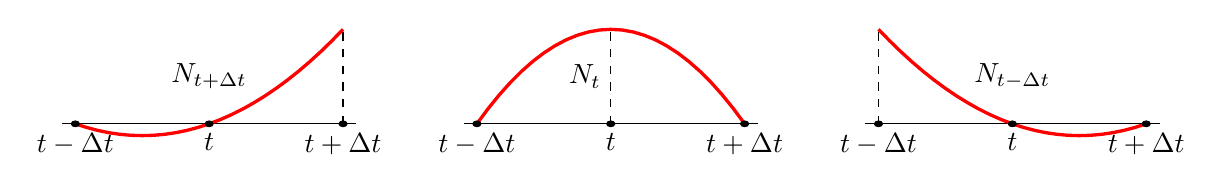
\begin{tikzpicture}[xscale=1.7,yscale=1.2]
\draw [thin] (-1.1,0) -- (1.1,0);
\draw [thin,dashed] (1,0)--(1,1);
\draw [red,very thick,domain = -1:1] plot (\x,{\x*(1+\x)/2});
\draw [thin,fill] (-1,0) circle [radius = 0.03];
\draw [thin,fill] (0,0) circle [radius = 0.03];
\draw [thin,fill] (1,0) circle [radius = 0.03];
\node [below] at (-1,0) {$t-\Delta t$};
\node [below] at (0,0) {$t$};
\node [below] at (1,0) {$t+\Delta t$};
\node at (0,0.5) {$N_{t+\Delta t}$};
%=============================================
\draw [thin] (1.9,0) -- (4.1,0);
\draw [thin,dashed] (3,0)--(3,1);
\draw [red,very thick,domain = 2:4] plot (\x,{(1-(\x-3))*(1+(\x-3))});
\draw [thin,fill] (2,0) circle [radius = 0.03];
\draw [thin,fill] (3,0) circle [radius = 0.03];
\draw [thin,fill] (4,0) circle [radius = 0.03];
\node [below] at (2,0) {$t-\Delta t$};
\node [below] at (3,0) {$t$};
\node [below] at (4,0) {$t+\Delta t$};
\node [left] at (3,0.5) {$N_{t}$};
%=============================================
\draw [thin] (4.9,0) -- (7.1,0);
\draw [thin,dashed] (5,0)--(5,1);
\draw [red,very thick,domain = 5:7] plot (\x,{-(\x-6)*(1-(\x-6))/2});
\draw [thin,fill] (5,0) circle [radius = 0.03];
\draw [thin,fill] (6,0) circle [radius = 0.03];
\draw [thin,fill] (7,0) circle [radius = 0.03];
\node [below] at (5,0) {$t-\Delta t$};
\node [below] at (6,0) {$t$};
\node [below] at (7,0) {$t+\Delta t$};
\node at (6,0.5) {$N_{t-\Delta t}$};
\end{tikzpicture}
\bicaption[Fig:NewmarkShapFun]{}{$N_{t+\Delta t},N_t,N_{t-\Delta t}$二次形函数}{Fig.$\!$}{Parabolic shape functions}
\end{figure}

于是,经过上述计算可以得到类似于(\ref{eq:NewmarkDisF})的表达式。进一步,若作如下参数规定
\begin{subequations}
\begin{align}
\gamma&=\frac{\int_{-1}^1W(t)\xi d\xi}{\int_{-1}^1W(t)d\xi}+\frac12\\
\beta&=\frac{\frac{1}{2}\int_{-1}^1W(t)\xi(1+\xi)d\xi}{\int_{-1}^1W(t)d\xi}
\end{align}
\end{subequations}
则,推导得到的关系将与等式(\ref{eq:NewmarkDisF})一致,意味着得到了Newmark算法。特别地,表\ref{Tab:NewWeighFun}给出了选择不同的权重函数$W(t)$时,将分别得到不同参数$\beta,\gamma$所对应的积分算法。从表\ref{Tab:NewWeighFun}可以发现,当$\gamma=\frac{1}{2}$时,所对应的权重函数都是对称的。
\vspace{-0.5cm}
\begin{table}[htbp]
\bicaption[Tab:NewWeighFun]{}{Newmark算法成员所对应的权重函数$W(t)$}{Table$\!$}{The weighted function $W(t)$ for some members of the Newmark family}
\vspace{0.5em}\centering\wuhao
\begin{tabular}{cccc}
\toprule[1.5pt]
$\gamma$&$\beta$&名称& $W(t)$\\
\midrule[1pt]
$\displaystyle-\frac12$ & $\displaystyle 0$ & $--$ & 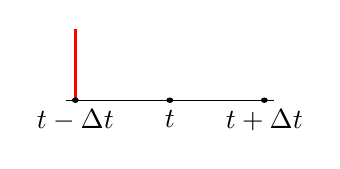
\begin{tikzpicture}[xscale=1.2,yscale=0.9]
\draw [thin] (-1.1,0) -- (1.1,0);
\draw [very thick,red] (-1,0)--(-1,1);
\draw [thin,fill] (-1,0) circle [radius = 0.03];
\draw [thin,fill] (0,0) circle [radius = 0.03];
\draw [thin,fill] (1,0) circle [radius = 0.03];
\node [below] at (-1,0) {$t-\Delta t$};
\node [below] at (0,0) {$t$};
\node [below] at (1,0) {$t+\Delta t$};
\end{tikzpicture}\\
$\displaystyle\frac12$ & $\displaystyle 0$ & 中心差分法 & 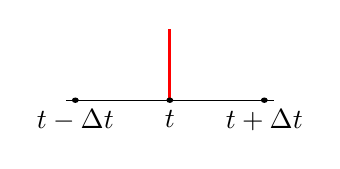
\begin{tikzpicture}[xscale=1.2,yscale=0.9]
\draw [thin] (-1.1,0) -- (1.1,0);
\draw [very thick,red] (0,0)--(0,1);
\draw [thin,fill] (-1,0) circle [radius = 0.03];
\draw [thin,fill] (0,0) circle [radius = 0.03];
\draw [thin,fill] (1,0) circle [radius = 0.03];
\node [below] at (-1,0) {$t-\Delta t$};
\node [below] at (0,0) {$t$};
\node [below] at (1,0) {$t+\Delta t$};
\end{tikzpicture}\\
$\displaystyle\frac32$ & $\displaystyle 1$ & 向后微分公式 & 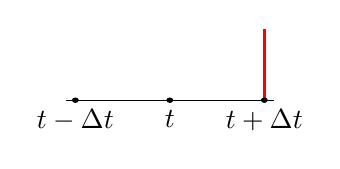
\begin{tikzpicture}[xscale=1.2,yscale=0.9]
\draw [thin] (-1.1,0) -- (1.1,0);
\draw [very thick,red] (1,0)--(1,1);
\draw [thin,fill] (-1,0) circle [radius = 0.03];
\draw [thin,fill] (0,0) circle [radius = 0.03];
\draw [thin,fill] (1,0) circle [radius = 0.03];
\node [below] at (-1,0) {$t-\Delta t$};
\node [below] at (0,0) {$t$};
\node [below] at (1,0) {$t+\Delta t$};
\end{tikzpicture} \\
$\displaystyle\frac12$ & $\displaystyle\frac{1}{12}$ & Fox-Goodwin格式 & 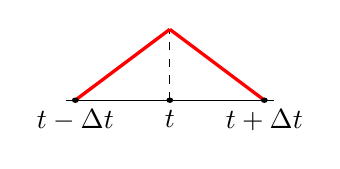
\begin{tikzpicture}[xscale=1.2,yscale=0.9]
\draw [thin] (-1.1,0) -- (1.1,0);
\draw [thin,dashed] (0,0)--(0,1);
\draw [red,very thick,domain = -1:0] plot (\x,{\x+1});
\draw [red,very thick,domain = 0:1] plot (\x,{1-\x});
\draw [thin,fill] (-1,0) circle [radius = 0.03];
\draw [thin,fill] (0,0) circle [radius = 0.03];
\draw [thin,fill] (1,0) circle [radius = 0.03];
\node [below] at (-1,0) {$t-\Delta t$};
\node [below] at (0,0) {$t$};
\node [below] at (1,0) {$t+\Delta t$};
\end{tikzpicture} \\
%$1/2$ & $1/10$ & Wilson-$\theta$($\theta=1.0$) & 2 & $\Omega_{cr}\le2\sqrt{3}$\\
$\displaystyle\frac12$ & $\displaystyle\frac16$ & 线平均加速度法 & 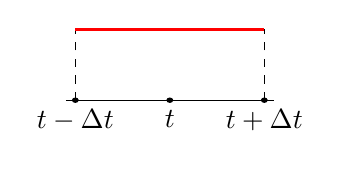
\begin{tikzpicture}[xscale=1.2,yscale=0.9]
\draw [thin] (-1.1,0) -- (1.1,0);
\draw [thin,dashed] (-1,0)--(-1,1);
\draw [thin,dashed] (1,0)--(1,1);
\draw [red,very thick,domain = -1:1] plot (\x,{1});
\draw [thin,fill] (-1,0) circle [radius = 0.03];
\draw [thin,fill] (0,0) circle [radius = 0.03];
\draw [thin,fill] (1,0) circle [radius = 0.03];
\node [below] at (-1,0) {$t-\Delta t$};
\node [below] at (0,0) {$t$};
\node [below] at (1,0) {$t+\Delta t$};
\end{tikzpicture} \\
$\displaystyle\frac12$ & $\displaystyle\frac14$ & 常平均加速度法/Trapeoidal规则 & 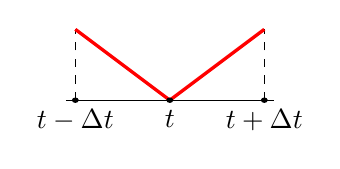
\begin{tikzpicture}[xscale=1.2,yscale=0.9]
\draw [thin] (-1.1,0) -- (1.1,0);
\draw [thin,dashed] (-1,0)--(-1,1);
\draw [thin,dashed] (1,0)--(1,1);
\draw [red,very thick,domain = -1:0] plot (\x,{-\x});
\draw [red,very thick,domain = 0:1] plot (\x,{\x});
\draw [thin,fill] (-1,0) circle [radius = 0.03];
\draw [thin,fill] (0,0) circle [radius = 0.03];
\draw [thin,fill] (1,0) circle [radius = 0.03];
\node [below] at (-1,0) {$t-\Delta t$};
\node [below] at (0,0) {$t$};
\node [below] at (1,0) {$t+\Delta t$};
\end{tikzpicture} \\
$\displaystyle\frac12$ & $\displaystyle\frac{1}{10}$ & $--$ & 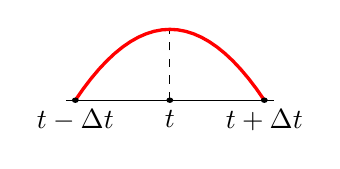
\begin{tikzpicture}[xscale=1.2,yscale=0.9]
\draw [thin] (-1.1,0) -- (1.1,0);
\draw [thin,dashed] (0,0)--(0,1);
\draw [red,very thick,domain = -1:1] plot (\x,{1-\x*\x});
\draw [thin,fill] (-1,0) circle [radius = 0.03];
\draw [thin,fill] (0,0) circle [radius = 0.03];
\draw [thin,fill] (1,0) circle [radius = 0.03];
\node [below] at (-1,0) {$t-\Delta t$};
\node [below] at (0,0) {$t$};
\node [below] at (1,0) {$t+\Delta t$};
\end{tikzpicture}\\
$\displaystyle\frac{3}{2}$ & $\displaystyle\frac45$ & Galerkin方法 & 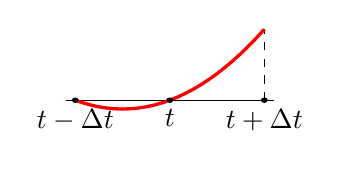
\begin{tikzpicture}[xscale=1.2,yscale=0.9]
\draw [thin] (-1.1,0) -- (1.1,0);
\draw [thin,dashed] (1,0)--(1,1);
\draw [red,very thick,domain = -1:1] plot (\x,{\x*(1+\x)/2});
\draw [thin,fill] (-1,0) circle [radius = 0.03];
\draw [thin,fill] (0,0) circle [radius = 0.03];
\draw [thin,fill] (1,0) circle [radius = 0.03];
\node [below] at (-1,0) {$t-\Delta t$};
\node [below] at (0,0) {$t$};
\node [below] at (1,0) {$t+\Delta t$};
\end{tikzpicture}\\
\bottomrule[1.5pt]
\end{tabular}
\end{table}

当使用更多的时间节点时,该有限元-加权残差方法可以推导出更高阶的算法格式。文\inlinecite{Zienkiewicz1977a}中给出了时间节点$t-2\Delta t,t-\Delta t,t,t+\Delta t$四个节点的使用三次多项式插值的离散格式。其算法格式为
\begin{equation}
\begin{aligned}
&[M(\gamma-1)+(\frac12\beta-\gamma+\frac13)\Delta tC+(\frac16\alpha-\frac12\beta+\frac13\gamma)\Delta t^2K]{^{t+\Delta t}\!U}\\
&\qquad+[(4-3\gamma)M+(4\gamma-\frac32\beta-\frac32)\Delta tC+(2\beta-\frac12\alpha-\frac32\gamma)\Delta t^2K]{^t\!U}\\
&\qquad+[(3\gamma-5)M+(\frac32-5\gamma+3)\Delta tC+(\frac12\alpha-\frac52\beta+3\gamma)\Delta t^2K]{^{t-\Delta t}\!U}\\
&\qquad+[(2-\gamma)M+(2\gamma-\frac{1}{2}\beta-\frac{11}{6})\Delta tC+(\beta-\frac16\alpha-\frac{11}{6}\gamma+1)\Delta t^2K]{^{t-2\Delta t}\!U}\\
&\qquad+(\frac16\alpha-\frac12\beta+\frac13\gamma){^{t+\Delta t}\!F}\Delta t^2+(2\beta-\frac12\alpha-\frac32\gamma){^t\!F}\Delta t^2\\
&\qquad+(\frac12\alpha-\frac52\beta+3\gamma){^{t-\Delta t}\!F}\Delta t^2+(\beta+1-\frac16\alpha-\frac{11}{6}\gamma){^{t-2\Delta t}\!F}\Delta t^2
\end{aligned}\label{eq:ZienANewLook13}
\end{equation}
其中,参数$\alpha,\beta,\gamma$被定义如下
\begin{equation}
\left\{\begin{aligned}
\alpha&=\frac{\int_0^3W\xi^3d\xi}{\int_0^3Wd\xi}\\
\beta&=\frac{\int_0^3W\xi^2d\xi}{\int_0^3Wd\xi}\\
\gamma&=\frac{\int_0^3W\xi d\xi}{\int_0^3Wd\xi}
\end{aligned}\right.
\end{equation}

有意思的是,当权重函数$W(t)$使用在$t+\Delta t$时刻的单位脉冲函数时,有参数$\alpha=27,\beta=9,\gamma=3$,可以得到Houbolt算法\cite{Houbolt1950}。而当参数满足如下关系时
\begin{equation}
\left\{\begin{aligned}
\alpha&=2+4\theta+3\theta^2+\theta^3\\
\beta&=\frac43+2\theta+\theta^2\\
\gamma&=1+\theta
\end{aligned}\right.
\end{equation}
算法格式(\ref{eq:ZienANewLook13})将退化为Wilson-$\theta$法。

文\inlinecite{Zienkiewicz1977a}中也考虑了在分段线性时间元的离散,而离散的形函数更加一般化,亦即在时刻$t+i\Delta t$有$W_{t+i\Delta t}=1$,其他时刻为均为零。其分段线性时间元和形函数表示如图\ref{Fig:NewmarkGenShapFun}。
\begin{figure}[htpb]
\centering
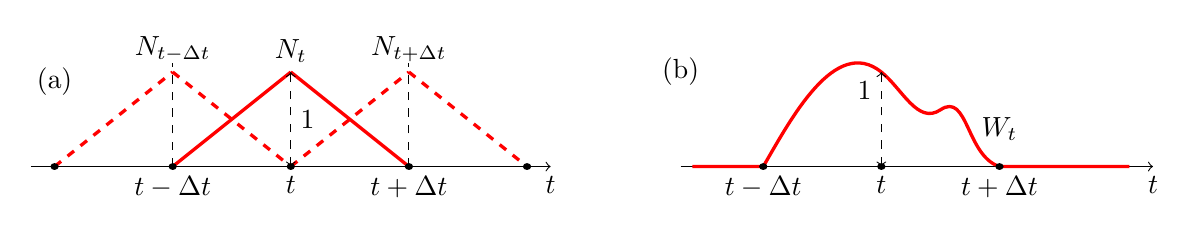
\begin{tikzpicture}[xscale=1.5,yscale=1.2]
\draw [thin,->] (-2.2,0) -- (2.2,0) node [below] {$t$};
\draw [thin,dashed] (-1,0)--(-1,1.1);
\draw [thin,dashed] (1,0)--(1,1.1);
%============================================
\draw [red,very thick,domain =-1:0] plot (\x,{\x+1});
\draw [red,very thick,domain =0:1] plot (\x,{-\x+1});
\draw [red,dashed,very thick,domain =-2:-1] plot (\x,{\x+2});
\draw [red,dashed,very thick,domain =-1:0] plot (\x,{-\x});
\draw [red,dashed,very thick,domain =0:1] plot (\x,{\x});
\draw [red,dashed,very thick,domain =1:2] plot (\x,{-\x+2});
%=============================================
\draw [thin,dashed,<->] (0,0)--(0,1);
%===============================================
\draw [thin,fill] (-2,0) circle [radius = 0.03];
\draw [thin,fill] (-1,0) circle [radius = 0.03];
\draw [thin,fill] (0,0) circle [radius = 0.03];
\draw [thin,fill] (1,0) circle [radius = 0.03];
\draw [thin,fill] (2,0) circle [radius = 0.03];
%=========================================
\node [below] at (-1,0) {$t-\Delta t$};
\node [below] at (0,0) {$t$};
\node [below] at (1,0) {$t+\Delta t$};
\node [above] at (-1,1) {$N_{t-\Delta t}$};
\node [above] at (0,1) {$N_{t}$};
\node [above] at (1,1) {$N_{t+\Delta t}$};
\node [right] at (0,0.5) {$1$};
\node at (-2,0.9) {(a)};
%**************************************************
\draw [thin,->] (3.3,0) -- (7.3,0) node [below] {$t$};
\draw [very thick,red] (3.4,0) -- (4,0) to [out=65,in=135] (5,1) to [out=-45,in=220] (5.5,0.6) to [out=40,in=158] (6,0) -- (7.1,0);
\draw [thin,dashed,<->] (5,0) -- (5,1) node [below left] {$1$};
\draw [thin,fill] (4,0) circle [radius = 0.03];
\draw [thin,fill] (5,0) circle [radius = 0.03];
\draw [thin,fill] (6,0) circle [radius = 0.03];
\node [below] at (4,0) {$t-\Delta t$};
\node [below] at (5,0) {$t$};
\node [below] at (6,0) {$t+\Delta t$};
\node at (6,0.4) {$W_{t}$};
\node at (3.3,1) {(b)};
\end{tikzpicture}
\bicaption[Fig:NewmarkGenShapFun]{}{(a):$N_{t+\Delta t},N_t,N_{t-\Delta t}$分段线性的形函数;(b):一般性的加权函数$W(t)$示意图}{Fig.$\!$}{(a):The piecewise linear shape functions;(b):The general weighting function $W(t)$}
\end{figure}

然后在一个更大的时间域$[0,m\Delta t]$上进行加权残差积分后得到
\begin{equation}
\begin{aligned}
&[M+\gamma_2\Delta tC+\beta_2\Delta t^2K]{^{t+\Delta t}\!U}\\
&\qquad+[-2M+(\gamma_1-\gamma_2)\Delta tC+(\beta_1-\beta_2+\gamma_2)\Delta t^2K]{^t\!U}\\
&\qquad+[M-\gamma_1\Delta tC+(\gamma_1-\beta_1)\Delta t^2K]{^{t-\Delta t}\!U}\\
&\qquad+\beta_2{^{t+\Delta t}\!F}\Delta t^2+(\beta_1-\beta_2+\gamma_2){^t\!F}\Delta t^2+(\gamma_1-\beta_1){^{t-\Delta t}\!F}\Delta t^2=0
\end{aligned}\label{eq:ZienANew15}
\end{equation}
其中,
\begin{equation}
\left\{\begin{aligned}
\gamma_1&=\int_{n-1}^nWd\xi \qquad \gamma_2=\int_{n}^{n+1}Wd\xi\\
\beta_1&=\int_{n-1}^nW\xi d\xi \qquad \beta_2=\int_{n}^{n+1}W\xi d\xi
\end{aligned}\right.
\end{equation}
这里的$n-1,n,n+1$分别代表$t-\Delta t,t,t+\Delta t$时刻,后文也将继续这样进行混用而不再特别指明,一般情况下是很容易分清的。当参数满足
\begin{equation}
\begin{aligned}
\gamma_2&=\gamma\qquad\beta_2=\beta\\
\gamma_1&=1-\gamma\quad \beta_1=\frac12-\beta
\end{aligned}
\end{equation}
算法格式(\ref{eq:ZienANew15})将退化为经典的Newmark算法(\ref{eq:NewmarkDisF})。同时,对算法(\ref{eq:ZienANew15})进行相容性分析将使得四个独立的参数退化为两个。

需要特别指明的是,如果将上述有限元离散的加权残差方法应用到位移-速度场的一阶运动微分方程(\ref{eq:DynqFirstOrder}),则可以使用两个不同的加权函数$W_1(t),W_2(t)$进而推导出新的算法格式,如高阶导数的显式算法\cite{Hoff1990,Hoff1990a}。



























最后,需要说明的是对于Newmark算法的位移和速度更新格式是现阶段直接积分法中使用最为广泛的更新格式。后续很多学者基于此提出了许多新的积分算法\cite{Hilber1978,Hilber1977,Wood1980a,KaiPing2008}。
 
\subsection{Wilson-$\theta$法}

Wilson-$\theta$法\cite{Wilson1968}是第一个无条件稳定的带可控数值耗散的积分算法,其本质上是平均加速度法的拓展。该算法假设在时间区间$(t_n,t_{n}+\theta\Delta t)$内,加速度线性变换,即
\begin{equation}
{^{t+\tau}\!\ddot{U}}={^t\!\ddot{U}}+\frac{\tau}{\theta\Delta t}({^{t+\Delta t}\!\ddot{U}}-{^t\!\ddot{U}})\label{eq:Tamma13.77}
\end{equation}
其中,$\theta$为自由参数,控制着算法的稳定性和精度,并且$0\le\tau\le\theta\Delta t$。在区间内对等式(\ref{eq:Tamma13.77})向变量$\tau$积分两次得到
\begin{subequations}
\begin{align}
{^{t+\tau}\!\dot{U}}&={^t\!\dot{U}}+{^t\!\ddot{U}}\tau+\frac{\tau^2}{2\theta\Delta t}({^{t+\theta}\!\ddot{U}}-{^t\!\ddot{U}})\\
{^{t+\tau}\!U}&={^t\!U}+{^t\!\dot{U}}\tau+\frac{1}{2}{^t\!\ddot{U}}\tau^2+\frac{1}{6\theta\Delta t}\tau^3({^{t+\theta}\!\ddot{U}}-{^t\!\ddot{U}})
\end{align}\label{eq:Tamma13.79}
\end{subequations}
其中,${^{t+\tau}\!U}=U(t_n+\tau)$并且${^{t+\theta}\!U}=U(t_n+\theta\Delta t)$。在上两式中雇佣$\tau=\theta\Delta t$并使用在$t+\theta\Delta t$时刻的平衡运动方程可得Wilson-$\theta$的算法格式如下
\begin{subequations}
\begin{align}
M{^{t+\theta\Delta t}\!\ddot{U}}+C{^{t+\theta\Delta t}\!\dot{U}}+K{^{t+\theta\Delta t}\!U}&={^{t+\theta\Delta t}\!F}\\
{^{t+\theta\Delta t}\!\ddot{U}}&=\frac{6}{\theta^2\Delta t^2}({^{t+\theta\Delta t}\!U}-{^t\!U})-\frac{6}{\theta}{^t\!\dot{U}}-2{^t\!\ddot{U}}\\
{^{t+\theta\Delta t}\!\dot{U}}&=\frac{3}{\theta\Delta t}({^{t+\theta\Delta t}\!U}-{^t\!U})-2{^t\!\dot{U}}-\frac{\theta\Delta t}{2}{^t\!\ddot{U}}
\end{align}\label{ee:Tammma13.80}
\end{subequations}
其中,${^{t+\theta\Delta t}\!F}={^t\!F}+\theta({^{t+\Delta t}\!F}-{^t\!F})$代表荷载的线性逼近。将Wilson-$\theta$改写为线性多步法的形式即有
\begin{equation}
\begin{split}
&\left[\frac{6}{\theta^2\Delta t^2}M+\frac{3}{\theta\Delta t}C+K\right]{^{t+\theta\Delta t}\!U}={^t\!F}+\theta({^{t+\Delta t}\!F}-{^t\!F})\\
&\qquad\qquad+M\left[\frac{6}{\theta^2\Delta t^2}{^t\!U}+\frac{6}{\theta\Delta t}{^t\!\dot{U}}+2{^t\!\ddot{U}}\right]+C\left[\frac{3}{\theta\Delta t}{^t\!U}+2{^t\!\dot{U}}+\frac{\theta\Delta t}{2}{^t\!\ddot{U}}\right]
\end{split}
\end{equation}
在计算得到了${^{t+\theta\Delta t}\!U}$之后,经过等式(\ref{ee:Tammma13.80})就可以计算得到${^{t+\theta\Delta t}\!\dot{U}}$和${^{t+\theta\Delta t}\!\ddot{U}}$。进而由等式(\ref{eq:Tamma13.79})在$\tau=\Delta t$时计算得到在$t+\Delta t$时刻的位移和速度。即
\begin{subequations}
\begin{align}
{^{t+\Delta t}\!\ddot{U}}&=\frac{6}{\theta^3\Delta t^2}({^{t+\theta\Delta t}\!U}-{^t\!U})-\frac{6}{\theta^2\Delta t}{^t\!\dot{U}}+\left(1-\frac{3}{\theta}\right){^t\!\ddot{U}}\\
{^{t+\Delta t}\!\dot{U}}&={^t\!\dot{U}}+\frac{\Delta t}{2}({^{t+\Delta t}\!\ddot{U}}+{^t\!\ddot{U}})\\
{^{t+\Delta t}\!U}&={^t\!U}+{^t\!\dot{U}}\Delta t+\frac{\Delta t^2}{6}({^{t+\Delta t}\!\ddot{U}}+2{^t\!\ddot{U}})
\end{align}
\end{subequations}

Wilson-$\theta$法是一个隐式算法。该算法是自启动的,不需要引入额外的启动机制。同时当$\theta=1$时,对应Newmark算法家族的线性加速度法;当$\theta\ge1.37$时,算法是无条件稳定的,一般$\theta$取值为1.4。Wilson-$\theta$实现二阶精度,且为带有可控的数值耗散,其耗散能力由参数$\theta$控制。但当$\theta>2$时,算法将减小数值耗散,同时增加相对周期误差。特别需要提及的是Wilson-$\theta$法很严重的超调行为\cite{Zhou2004c},具体地,存在位移上的二阶超调和速度上的一阶超调行为。这也是该算法最大的一个缺点。有意思的是,文\inlinecite{Mohammadzadeh2017}中通过引入一个结构依赖性的参数$\alpha$可以很好的处理Wilson-$\theta$的超调行为,而且文\inlinecite{Benitez2013}也分析了Wilson-$\theta$法严重的超调行为是由于初值加速度的不协调引起的,如果引入协调的初始加速度,该算法也将没有超调行为。

\subsection{Park算法}
Park算法是一个线性多步算法。它是隐式的、无条件稳定的二阶精度算法。而且带有渐进消弭特性,因此是L-稳定的。类似于Houbolt算法,Park算法也是基于在$t+\Delta t$的平衡运动方程和两个向后微分公式逼近速度和加速度得到。其算法格式描述如下
\begin{subequations}
\begin{align}
M{^{t+\Delta t}\!\ddot{U}}+C{^{t+\Delta t}\!\dot{U}}+K{^{t+\Delta t}\!U}&={^{t+\Delta t}\!F}\\
{^{t+\Delta t}\!\dot{U}}&=\frac{1}{6\Delta t}(10{^{t+\Delta t}\!U}-15{^{t}\!U}+6{^{t-\Delta t}\!U}-{^{t-2\Delta t}\!U})\\
{^{t+\Delta t}\!\ddot{U}}&=\frac{1}{6\Delta t}(10{^{t+\Delta t}\!\dot{U}}-15{^{t}\!\dot{U}}+6{^{t-\Delta t}\!\dot{U}}-{^{t-2\Delta t}\!\dot{U}})
\end{align}
\end{subequations}

该算法是刚性稳定的。除此之外,Park算法也可以通过Gear两步法\cite{Gear1971a}和三步刚性稳定算法\cite{Gear1971a}结合产生。因此该算法可以使用较大的时间步长求解刚性系统。它也拥有在高频段的强数值耗散,但在低频段其耗散较Houbolt算法低,同时也提高了相对周期误差。对于一阶微分系统(\ref{eq:firstSystem})的线性多步法公式(\ref{eq:firstsystemLMS}),Park算法对应的参数取值为$(k=3)$
\begin{equation}
\begin{split}
\alpha_0&=10,\alpha_1=-15,\alpha_2=6,\alpha_3=-1\\
\beta_0&=6,\beta_1=\beta_2=\beta_3=0
\end{split}
\end{equation}

\subsection{Hilber-Hughes-Taylor-$\alpha$算法}
Hilber-Hughes-Taylor-$\alpha$算法(HHT-$\alpha$)\cite{Hilber1977}是基于设计无条件稳定的带可控数值耗散的直接积分法。该算法在时间区间$[t_n,t_{n+1}]$内使用Newmark格式的位移和速度的更新公式,也就是说Newmark格式是被使用作为一个基础和起始点。即:
\begin{subequations}
\begin{align}
{^{t+\Delta t}\!{U}}&={^t\!U}+{^t\!\dot{U}}\Delta t+\frac{\Delta t^2}{2}[(1-2\beta){^t\!\ddot{U}}+2\beta{^{t+\Delta t}\!\ddot{U}}]\\
{^{t+\Delta t}\!\dot{U}}&={^t\!\dot{U}}+\Delta t[(1-\gamma){^t\!\ddot{U}}+\gamma{^{t+\Delta t}\!\ddot{U}}]
\end{align}\label{eq:HHTUV}
\end{subequations}
并且离散的平衡方程被加权满足,即
\begin{equation}
M{^{t+\Delta t}\!\ddot{U}}+(1-\alpha)C{^{t+\Delta t}\!\dot{U}}+\alpha C{^{t}\!\dot{U}}+(1-\alpha)K{^{t+\Delta t}\!U}+\alpha K{^t\!U}={^{t+\alpha}\!F}
\end{equation}
对于外荷载的激励加权值${^{t+\alpha}\!F}$通常情况下可以选择为线性叠加,即
\begin{equation}
{^{t+\alpha}\!F}=(1-\alpha){^{t+\Delta t}\!F}+\alpha{^t\!F}
\end{equation}
但需要说明的是,文\inlinecite{Erlicher2002}中还分析了另外y一种组合方式的影响。即
\begin{align}
{^{t+\alpha}\!F}=F((1-\alpha)t_{n+1}+\alpha t_n)
\end{align}

将位移和速度更新公式带入加权组合的离散运动方程,可得
\begin{equation}
\begin{split}
&\left[M+\Delta t\gamma(1-\alpha)C+\Delta t^2\beta(1-\alpha)K\right]{^{t+\Delta t}\!\ddot{U}}\\
&\qquad\qquad=-(1-\alpha)C{^{t+\Delta t}\!\widetilde{\dot{U}}}-\alpha C{^t\!\dot{U}}+(1-\alpha)K{^{t+\Delta t}\!\widetilde{U}}-\alpha K{^t\!U}+{^{t+\alpha}\!F}
\end{split}
\end{equation}
其中,${^{t+\Delta t}\!\widetilde{\dot{U}}}$和${^{t+\Delta t}\!\widetilde{U}}$来自于等式(\ref{eq:NewmarkUVW})。于是,下一时刻的加速度可由求解上式得到,而下一时刻的位移和速度则有等式(\ref{eq:HHTUV})计算得到。

HHT-$\alpha$算法是隐式的、二阶精度算法。当下列参数满足时,可实现无条件稳定性:
\begin{equation}
-\frac{1}{3}\le\alpha\le0,\quad\beta=\frac{(1-\alpha)^2}{4}\quad\text{和}\quad\gamma=\frac{1}{2}-\alpha
\end{equation}
其中,参数$\alpha$控制算法的耗散特性。$\alpha$取更大的负值将增加数值耗散和相对周期误差;相反,取更小的负值将会减小耗散和相对周期误差。无论情况下,其数值耗散和相对周期误差都比Houbolt算法和Wilson-$\theta$算法低。同时,它并不是最优的耗散性算法。除此之外,它具有速度上的一阶超调行为。
\subsection{Wood-Bosak-Zienkiewicz-$\alpha$算法}
Wood-Bosak-Zienkiewicz-$\alpha$算法(WBZ-$\alpha$)\cite{Wood1980a}是基于HHT-$\alpha$法的思想,修改了加权平衡方程的惯性力项,即保持Newmar的位移和速度更新公式不变,使用如下的加权平衡方程
\begin{equation}
(1-\alpha)M{^{t+\Delta t}\!\ddot{U}}+\alpha M{^{t+\Delta t}\!\ddot{U}}+C{^{t+\Delta t}\!\dot{U}}+K{^{t+\Delta t}\!U}={^{t+\Delta t}\!F}
\end{equation}
其中$\alpha$为算法参数。仍将Newmark算法的位移和速度更新公式(\ref{eq:HHTUV})带入上式得到
\begin{equation}
\left[(1-\alpha)M+\Delta t\gamma C+\Delta t^2\beta K\right]{^{t+\Delta t}\!\ddot{U}}={^{t+\Delta t}\!F}-\alpha M{^{t}\!\ddot{U}}-C{^{t+\Delta t}\!\widetilde{\dot{U}}}-K{^{t+\Delta t}\!\widetilde{U}}
\end{equation}
其中,${^{t+\Delta t}\!\widetilde{\dot{U}}}$和${^{t+\Delta t}\!\widetilde{U}}$来自于等式(\ref{eq:NewmarkUVW})。当参数满足如下条件时,WBZ-$\alpha$算法实现二阶精度和无条件稳定性:
\begin{equation}
\alpha\le0,\quad\gamma=\frac{1}{2}-\alpha\quad\text{和}\quad\beta=\frac{1}{4}(1-\alpha)^2
\end{equation}
WBZ-$\alpha$算法的数值特点类似于HHT-$\alpha$算法。如,不是最优的耗散性算法以及WBZ-$\alpha$也具有速度上的一阶超调行为。

\subsection{基于速度更新的$\gamma_s$格式}
Namburu和Tamma在20世纪90年代左右基于一般形式的守恒律微分方程的Lax-Wendroff/Taylor-Galerkin离散得到了一类速度更新的显式/隐式直接积分算法\cite{Tamma1988,Tamma1988c,Tamma1989,Tamma1990a,Tamma1990,Tamma1992,Namburu1992}。其中,具有一般表达性的是$\gamma_s$族算法\cite{Namburu1992}
\begin{align}
[M+\Delta t\gamma_1C+\Delta t^2\gamma_1\gamma_2K]{^{t+\Delta t}\!\dot{U}}&=[M-\Delta t(1-\gamma_1)C-\Delta t^2\gamma_1(1-\gamma_2)K]{^t\!\dot{U}}\notag\\
&\quad -\Delta tK{^t\!U}+\Delta t[(1-\gamma_1){^t\!F}+\gamma_1{^{t+\Delta t}\!F}]\\
{^{t+\Delta t}\!U}&={^t\!U}+\Delta t[\gamma_3{^{t+\Delta t}\!\dot{U}}+(1-\gamma_3){^t\!\dot{U}}]\label{eq:TammaU}
\end{align}

对于参数选取条件,在无阻尼情况下$\xi=0$时,
\begin{equation}
\gamma_1+\gamma_3=1\qquad 1-2\gamma_1=0
\end{equation}
可保证实现二阶精度。
在有阻尼时,仅需要$\gamma_1+\gamma_3=1$即可。

同时,对于具体的参数取值,原文\inlinecite{Namburu1992}给出如下情况($0\le\xi\le1$)
\begin{itemize}
\item[\ddag] 当$\gamma_1=\gamma_2=\gamma_3=\frac{1}{2}$时,可以实现无条件稳定的二阶隐式算法\cite{Tamma1990}。
\item[\ddag] 当$\gamma_1=\gamma_3=\frac{1}{2},\gamma_2<0.5$时,可以实现条件稳定的二阶隐式算法。
\item[\ddag] 当$\gamma_1=\gamma_3=\frac{1}{2},\gamma_2=0$时,可以实现条件稳定的二阶显式算法\cite{Tamma1988,Tamma1988c,Tamma1989,Tamma1990a,Tamma1992},其稳定域为$\Omega_{cr}=2$。
\end{itemize}

对于无阻尼的线性守恒系统,上述算法是能量、动量以及角动量守恒的。该格式的原始性工作由Simo和Tarnow针对非线性系统在位移-速度场中提出\cite{Simo1992b}。

\textbf{非线性的应用} 上述格式在求解非线性动力学方程时,可采用如下更具一般性的算法格式\cite{Tamma1993}
\begin{equation}
M{^{t+\Delta t}\!\Delta \dot{U}}=\Delta t({^{t+\Delta t/2}\!F_{int}}+{^{t+\Delta t/2}\!F_{ext}})\label{eq:Tamma1992}
\end{equation}
而位移更新公式则仍使用公式(\ref{eq:TammaU})。实现上,上述方程的物理含义就是:\textbf{系统动量的增量($M\Delta \dot{U}$)等于系统所受到外力的冲量(和$\Delta tF_{\text{合}}$)}。
其中,$F_{int}$和$F_{ext}$分别为系统的内力和外力。对于线性系统,二者可分别看作$-C\dot{U}(t)-KU(t)$和$F(t)$。而上标$t+\Delta t/2$表示在$t+\Delta t/2$时刻进行计算。因此对于不同的内力和外力在$t+\Delta t/2$时刻的逼近表达式可以导出不同的积分格式。如采用下列等式计算
\begin{align}
{^{t+\Delta t/2}\!F_{int}}&=\frac{1}{2}[(-C{^t\!\dot{U}}-K{^t\!U})+(-C{^{t+\Delta t}\!\dot{U}}-K{^{t+\Delta t}\!U})]\\
{^{t+\Delta t/2}\!F_{ext}}&=\frac{1}{2}({^t\!F}+{^{t+\Delta t}\!F})
\end{align}
于是,算法格式(\ref{eq:Tamma1992})将导出$\gamma_1=\gamma_2=\gamma_3=\frac{1}{2}$的算法\cite{Tamma1990}。

该算法的一个主要特点是真正意义上的自启动算法,并不需要任何形式的初始加速度启动机制。
特别地,当上述参数依赖于结构的特性时,将导出一类依赖于结构的直接积分法。如后面的Soares-Jr型算法族。









\subsection{带中点加速度的中点公式}
对于如下形式的二阶精度的隐式算法\cite{JasonHar2012}(MPR-MPA)
\begin{subequations}
\begin{align}
\left[M+\frac{1}{2}C\Delta t+\frac{1}{4}K\Delta t^2\right]{^{t+\Delta t}\!\ddot{U}}&=-C{^t\!\dot{U}}-K\left[{^t\!U}+\frac{\Delta t}{2}{^t\!\dot{U}}\right]+\frac{1}{2}({^t\!F}+{^{t+\Delta t}\!F})\\
{^{t+\Delta t}\!U}&={^t\!U}+{^t\!\dot{U}}\Delta t+\frac{\Delta t^2}{2}{^{t+\Delta t}\!\ddot{U}}\\
{^{t+\Delta t}\!\dot{U}}&={^t\!\dot{U}}+\frac{\Delta t}{2}({^t\!\ddot{U}}+{^{t+\Delta t}\!\ddot{U}})
\end{align}
\end{subequations}

上式公式的加速度在时刻$t_{n+\frac{1}{2}}$严格成立。需要说明的是,在大多数非耗散性算法中,该算法的鲁棒性较好,而且在线性多步法的框架下是最佳选择。同时在位移和速度上都没有超调行为。

\subsection{三参数优化算法/CH-$\alpha$法}
在结构动力学数值响应求解算法中,使用最为广泛、研究最为深入的另外一个算法就是Chung和Hulbert提出的广义$\alpha$法(The generalized-$\alpha$ method)\cite{Chung1993}。特别地,为了与后续更加一般化的$\alpha$方法\cite{KaiPing2008}区别开来,本文都将该算法注释为:CH-$\alpha$算法。

事实上,在Chung和Hulbert等人提出CH-$\alpha$算法之前,国内的邵慧萍等人就已经提出了该算法,其算法命令为三参数优化算法\cite{邵慧萍1988}。其算法格式结合HHT-$\alpha$算法和WBZ-$\alpha$算法的特点,定义了如下的算法格式:
\begin{subequations}
\begin{align}
(1-\xi){^{t+\Delta t}\!F}+\xi{^t\!F}&=M[(1-\alpha){^{t+\Delta t}\!\ddot{U}}+\alpha {^t\!\ddot{U}}]+C[(1-\eta){^{t+\Delta t}\!\dot{U}}+\eta{^t\!\dot{U}}]\notag\\
&\qquad\qquad+K[(1-\delta){^{t+\Delta t}\!U}+\delta{^t\!U}]\\
{^{t+\Delta t}\!{U}}&={^t\!U}+{^t\!\dot{U}}\Delta t+\frac{\Delta t^2}{2}[(1-2\beta){^t\!\ddot{U}}+2\beta{^{t+\Delta t}\!\ddot{U}}]\\
{^{t+\Delta t}\!\dot{U}}&={^t\!\dot{U}}+\Delta t[(1-\gamma){^t\!\ddot{U}}+\gamma{^{t+\Delta t}\!\ddot{U}}]
\end{align}
\end{subequations}

显然,该三参数优化算法仍然雇用了Newmark算法的位移和速度更新公式。当参数取不同的值,将退化为前述提及的一些算法,如
\begin{itemize}
\item[\ddag] 当$\alpha=\delta=\eta=\xi=0$时,该算法退化为Newmark家族算法。
\item[\ddag] 当$\alpha=0$时,该算法退化为HHT-$\alpha$算法。
\item[\ddag] 当$\delta=\eta=\xi=0$时,该算法退化为WBZ-$\alpha$算法。
\end{itemize}

事实上,上述涉及的六个参数中,只有三个参数被选择以实现二阶精度和无条件稳定性。即
\begin{equation}
\left\{\begin{aligned}
\alpha\le\delta\le\frac{1}{2}&\qquad \beta\ge\frac{1}{2}\gamma=\frac{1}{2}(\frac{1}{2}-\alpha+\delta)\\
\eta=\xi=\delta&\qquad \xi\ge0
\end{aligned}\right.
\end{equation}

如果将这些参数与高频极限下的谱半径$\rho_{\infty}$相联系,则可以定义如下的单参数簇算法
\begin{equation}
\left\{\begin{aligned}
\alpha&=\frac{2\rho_{\infty}-1}{\rho_{\infty}+1}\\
\beta&=\frac{1}{(\rho_{\infty}+1)^2}\\
\gamma&=\frac{3-\rho_{\infty}}{2(1+\rho_{\infty})}\\
\eta&=\xi=\delta=\frac{\rho_{\infty}}{\rho_{\infty}+1}
\end{aligned}\right.
\end{equation}

\subsubsection{最优的$\chi$格式}
邵慧萍在文\inlinecite{邵慧萍1988}中给出了一组最优的$\chi$算法格式,其参数取值如下
\begin{equation}
\left\{\begin{aligned}
\alpha&=-\frac{2\rho_{\infty}-1}{\rho_{\infty}+1}\qquad\beta=-\frac{1}{(\rho_{\infty}+1)^2}\\
\gamma&=-\frac{3-\rho_{\infty}}{2(1+\rho_{\infty})}\qquad\eta=\xi=\delta=-\frac{\rho_{\infty}}{\rho_{\infty}+1}
\end{aligned}\right.
\end{equation}

\subsubsection{HHT-$\alpha$算法}
当上述算法被定义如下时,将退化为HHT-$\alpha$算法。
\begin{equation}
\left\{\begin{aligned}
\alpha&=0\qquad\qquad\qquad\beta=\frac{1}{(\rho_{\infty}+1)^2}\\
\gamma&=\frac{3-\rho_{\infty}}{2(1+\rho_{\infty})}\qquad\eta=\xi=\delta=\frac{\rho_{\infty}}{\rho_{\infty}+1}
\end{aligned}\right.
\end{equation}

\subsubsection{WBZ-$\alpha$算法}
当上述算法被定义如下时,将退化为WBZ-$\alpha$算法。
\begin{equation}
\left\{\begin{aligned}
\alpha&=\frac{\rho_{\infty}-1}{\rho_{\infty}+1}\quad\qquad\beta=-\frac{1}{(\rho_{\infty}+1)^2}\\
\gamma&=-\frac{3-\rho_{\infty}}{2(1+\rho_{\infty})}\qquad\eta=\xi=\delta=0
\end{aligned}\right.
\end{equation}

\subsubsection{CH-$\alpha$算法}
Chung和Hulbert于1993年在应用力学杂志发表了CH-$\alpha$算法\cite{Chung1993}。该算法实质上与前述的三参数优化算法一致。其算法的平衡方程加权组合如下
\begin{equation}
M{^{n+(1-\alpha_m)}\!\ddot{U}}+C{^{n+(1-\alpha_f)}\!\dot{U}}+K{^{n+(1-\alpha_f)}\!U}={^{n+(1-\alpha_f)}\!F}
\end{equation}
其中
\begin{subequations}
\begin{align}
{^{n+(1-\alpha_m)}\!\ddot{U}}&=(1-\alpha_m){^{t+\Delta t}\!\ddot{U}}+\alpha_m{^t\!\ddot{U}}\\
{^{n+(1-\alpha_f)}\!\dot{U}}&=(1-\alpha_f){^{t+\Delta t}\!\dot{U}}+\alpha_f{^t\!\dot{U}}\\
{^{n+(1-\alpha_f)}\!{U}}&=(1-\alpha_f){^{t+\Delta t}\!{U}}+\alpha_f{^t\!{U}}
\end{align}
\end{subequations}
对于外力荷载的加权组合${^{n+(1-\alpha_f)}\!F}$类似于三参数优化算法,有两种组合模式。其位移和速度更新公式使用Newmark算法的位移和速度更新公式(\ref{eq:HHTUV})。于前者一致的是,参数$\alpha_m=0$和$\alpha_f=0$分别对应着HHT-$\alpha$和WBZ-$\alpha$算法;而$\alpha_m=\alpha_f=0$对应于原始的Newmark家族算法。

当满足下列条件时,CH-$\alpha$算法实现二阶精度
\begin{equation}
\gamma=\frac{1}{2}-\alpha_m+\alpha_f
\end{equation}
而无条件稳定性要求
\begin{equation}
\alpha_m\le\alpha_f\le\frac{1}{2}\qquad\text{和}\qquad\beta\ge\frac{1}{4}+\frac{1}{2}(\alpha_f-\alpha_m)
\end{equation}

为了实现最优的数值耗散,算法在高频极限情况下的三个特征值$(\lambda_{1,2,3}^{\infty})$应满足下列条件
\begin{equation}
\text{Im} (\lambda_{1,2}^{\infty})=0\qquad|\lambda_{3}^{\infty}|=|\lambda_{1,2}^{\infty}|
\end{equation}
其中Im表示取复数的虚部。于是,参数$\beta$应满足
\begin{equation}
\beta=\frac{1}{4}(1-\alpha_m+\alpha_f)^2
\end{equation}

同样的,如果以高频极限下的谱半径值$\rho_{\infty}$表示算法的耗散特性,则CH-$\alpha$算法可以表示为
\begin{equation}
\alpha_m=\frac{2\rho_{\infty}-1}{\rho_{\infty}+1}\qquad\alpha_f=\frac{\rho_{\infty}}{\rho_{\infty}+1}
\end{equation}

当$\rho_{\infty}=1$时,CH-$\alpha$算法退化为非耗散性的带终点加速度的中点公式(MPR-EPA);而$\rho_{\infty}=0$退化为带有渐进消弭特性的WBZ-$\alpha$算法。特别地,CH-$\alpha$算法被证明是数值耗散特性最优的算法,同时也是存在虚假根的算法中,虚假根影响数值解最小的算法\cite{Hulbert1994}。

\subsection{广义$\alpha$算法}

尽管三参数优化算法/CH-$\alpha$算法具有很好的耗散特性,但是却存在速度上的一阶超调行为。因此,基于加权组合平衡方程引入数值耗散的思想,于开平教授于2008年提出了更具一般性的广义$\alpha$算法\cite{KaiPing2008}。该算法不仅使得前述的WBZ-$\alpha$、HHT-$\alpha$以及CH-$\alpha$算法都是该算法的一个特例,而且还分别提出了三个算法对应的无超调行为的新算法。其广义$\alpha$算法的算法描述如下
\begin{subequations}
\begin{align}
(1-\alpha)M{^{t+\Delta t}\!\ddot{U}}+\alpha M{^{t}\!\ddot{U}}+(1-\delta)C{^{t+\Delta t}\!\dot{U}}&+\delta C{^t\!\dot{U}}+(1-\eta)K{^{t+\Delta t}\!U}+\eta K{^t\!U}\notag\\
&=(1-\eta){^{t+\Delta t}\!F}+\eta {^t\!F}\\
{^{t+\Delta t}\!{U}}&={^t\!U}+{^t\!\dot{U}}\Delta t+\Delta t^2(\epsilon{^t\!\ddot{U}}+\beta{^{t+\Delta t}\!\ddot{U}})\\
{^{t+\Delta t}\!\dot{U}}&={^t\!\dot{U}}+\Delta t(\mu{^t\!\ddot{U}}+\gamma{^{t+\Delta t}\!\ddot{U}})
\end{align}
\end{subequations}

为了实现二阶精度,参数需要满足条件
\begin{equation}
\gamma+\mu=1\qquad\alpha+\beta+\epsilon-\eta-\mu=0\qquad\beta+\epsilon+\delta-\eta=\frac{1}{2}
\end{equation}
同时,无条件稳定性要求
\begin{equation}
\gamma\ge\frac{1}{2}\ge\eta\ge\delta\qquad\beta\ge\frac{1}{2}(\eta+\gamma-\delta)
\end{equation}

当分别满足以下三个条件时,可设计对应的三个算法
\begin{itemize}
\item[\ddag] Im$(\lambda_{1,2}^{\infty})=0$并且$|\lambda_3^{\infty}|=|\lambda_{1,2}^{\infty}|$时,可以得到最优的数值耗散性算法。
\item[\ddag] 算法在低频段的数值耗散尽可能小,即当$\omega\Delta t\to0$时,谱半径$\rho\to0$。此时,可设计出类似于HHT-$\alpha$算法。
\item[\ddag] 在高频极限下,其虚假根为0,即$\lambda_3^{\infty}\to0$。此时,可设计出类似于WBZ-$\alpha$算法。
\end{itemize}

特别地,参数$\mu$满足
\begin{equation}
\mu=\frac{\rho_{\infty}}{\rho_{\infty}+1}
\end{equation}
时,广义$\alpha$算法没有超调行为。
{}
其广义$\alpha$算法对应的不同算法成员如下表\ref{table2}所示
\vspace{-1cm}
\begin{table}[htbp]
\bicaption[table2]{}{广义$\alpha$积分算法成员的参数取值}{Table$\!$}{Algorithmic parameters of the generalized-$\alpha$ method family}
\vspace{0.5em}\centering\wuhao
\begin{tabular}{ccccccc}
\toprule[1.5pt]
参数 & NOCH-$\alpha$ & CH-$\alpha$ & NOHHT-$\alpha$ & HHT-$\alpha$ & NOWBZ-$\alpha$ & WBZ-$\alpha$\\
\midrule[1pt]
$\alpha$ & $\frac{2\rho_{\infty}-1}{\rho_{\infty}+1}$ & $\frac{2\rho_{\infty}-1}{\rho_{\infty}+1}$ & $0$ & $0$ & $\frac{\rho_{\infty}-1}{\rho_{\infty}+1}$ & $\frac{\rho_{\infty}-1}{\rho_{\infty}+1}$\\ [0.5em]
$\delta$ & $\frac{3\rho_{\infty}-1}{2(\rho_{\infty}+1)}$ & $\frac{\rho_{\infty}}{\rho_{\infty}+1}$ & $\frac{1-\rho_{\infty}}{2(\rho_{\infty}+1)}$ & $\frac{1-\rho_{\infty}}{\rho_{\infty}+1}$ & $\frac{\rho_{\infty}-1}{2(\rho_{\infty}+1)}$ & $0$\\ [0.5em]
$\eta$ & $\frac{\rho_{\infty}}{\rho_{\infty}+1}$ & $\frac{\rho_{\infty}}{\rho_{\infty}+1}$ & $\frac{1-\rho_{\infty}}{(\rho_{\infty}+1)}$ & $\frac{1-\rho_{\infty}}{(\rho_{\infty}+1)}$ & $0$ & $0$\\ [0.5em]
$\epsilon$ & $\frac{\rho_{\infty}}{(\rho_{\infty}+1)^2}$ & $\frac{\rho_{\infty}^2+2\rho_{\infty}-1}{2(\rho_{\infty}+1)^2}$ & $\frac{\rho_{\infty}}{(\rho_{\infty}+1)^2}$ & $\frac{\rho_{\infty}^2+2\rho_{\infty}-1}{2(\rho_{\infty}+1)^2}$ & $\frac{\rho_{\infty}}{(\rho_{\infty}+1)^2}$ & $\frac{\rho_{\infty}^2+2\rho_{\infty}-1}{2(\rho_{\infty}+1)^2}$\\ [0.5em]
$\beta$ & $\frac{1}{(\rho_{\infty}+1)^2}$ & $\frac{1}{(\rho_{\infty}+1)^2}$ & $\frac{1}{(\rho_{\infty}+1)^2}$ & $\frac{1}{(\rho_{\infty}+1)^2}$ & $\frac{1}{(\rho_{\infty}+1)^2}$ & $\frac{1}{(\rho_{\infty}+1)^2}$\\ [0.5em]
$\mu$ & $\frac{\rho_{\infty}}{\rho_{\infty}+1}$ & $\frac{3\rho_{\infty}-1}{2(\rho_{\infty}+1)}$ & $\frac{\rho_{\infty}}{\rho_{\infty}+1}$ & $\frac{3\rho_{\infty}-1}{2(\rho_{\infty}+1)}$ & $\frac{\rho_{\infty}}{\rho_{\infty}+1}$ & $\frac{3\rho_{\infty}-1}{2(\rho_{\infty}+1)}$\\ [0.5em]
$\gamma$ & $\frac{1}{\rho_{\infty}+1}$ & $\frac{3-\rho_{\infty}}{2(\rho_{\infty}+1)}$ & $\frac{1}{\rho_{\infty}+1}$ & $\frac{3-\rho_{\infty}}{2(\rho_{\infty}+1)}$ & $\frac{1}{\rho_{\infty}+1}$ & $\frac{3-\rho_{\infty}}{2(\rho_{\infty}+1)}$\\ [0.5em]
$\rho_{\infty}$ & $[0,1]$ & $[0,1]$ & $[0.5,1]$ & $[0.5,1]$ & $[0,1]$ & $[0,1]$\\
\bottomrule[1.5pt]
\end{tabular}
\end{table}

注意到NOCH-$\alpha$、NOHHT-$\alpha$和NOWBZ-$\alpha$是三个新的广义$\alpha$成员,其前缀“NO”表示在速度和位移上都没有超调行为。而且这三个算法满足Hughes所提出的一个具有竞争性算法的六个属性\cite{book:dover,Hilber1978}。










%%%%%%%%%%%%%%%%%%%%%%%%%%%%%%%%%%%%%%%%%%%%%%%%%%%%%%%%%%%%%%%%%%%%%%%%%%%%%%%%%%%%%%%%%%%%%%%%%%%%%%%%%%%
\section{加权残值法}
\subsection{$\rho$-算法}
$\rho$-算法\cite{Bazzi1982}是通过假设在时间区间$[t_n,t_{n+1}]$内的位移满足
\begin{equation}
U(t)=N_1(t){^t\!U}+N_2(t){^t\!\dot{U}}+N_3(t){^t\!\ddot{U}}+N_4(t){^{t+\Delta t}\!{U}}
\end{equation}
其中,$N_i(t),i=1,2,3,4$是时间域上的形函数,亦即表明上式实质上是进行了时间有限元的离散。同时,通过引入权重函数$W(t)\equiv1$在区间内进行残差积分,并限制其值为零。即
\begin{equation}
\int_{t_n}^{t_{n+1}}[M\ddot{U}(t)+C\dot{U}(t)+KU(t)-F(t)]=0
\end{equation}
经过复杂的计算\footnote{事实上,原文作者也是空降得到下面的计算格式,而且关于其增量的计算格式根据后文的精度分析反推可知有误,在此更正。},就可以得到如下的位移、速度和加速度的更新公式
\begin{subequations}
\begin{align}
{^{t+\Delta t}\!U}&={^t\!U}+\Delta U\\
{^{t+\Delta t}\!\dot{U}}&=-{^t\!\dot{U}}+\frac{1-\rho_{\infty}}{1+\rho_{\infty}}{^t\!\ddot{U}}\Delta t+\frac{2}{\Delta t}\Delta U\\
{^{t+\Delta t}\!\ddot{U}}&=\frac{(1+\rho_{\infty})(1+\rho_{\infty}^2)}{\Delta t^2}(\Delta U-{^t\!\dot{U}}\Delta t)+(1-\rho_{\infty}-\rho_{\infty}^3){^t\!\ddot{U}}
\end{align}
\end{subequations}
其位移的增量$\Delta U$的计算公式为
\begin{equation}
[M+\frac{\Delta t}{2}C+\frac{\Delta t^2}{2(\rho_{\infty}+1)}K]\Delta U=-\frac{1}{2}K{^t\!U}\Delta t^2+M{^t\!\dot{U}}\Delta t+\frac{\rho_{\infty}-1}{2(\rho_{\infty}+1)}M{^t\!\ddot{U}}\Delta t^2+\frac{\Delta t^2}{2}{^t\!F^*}
\end{equation}
其中,
\begin{equation}
{^t\!F^*}=\frac{1}{\Delta t}\int_{t_n}^{t_{n+1}}F(t)dt\label{eq:Bazzi11}
\end{equation}
表示在时间区间内的外力平均值。其参数$\rho_{\infty}$实质上表示算法在高频极限下的谱半径值,亦即表示算法的耗散能力大小。当$\rho_{\infty}=1$时,$\rho$-算法退化为Trapeoidal规则。

特别需要说明的是,$\rho$-算法在无阻尼情况下实现二阶精度;而在有阻尼情况仅有一阶精度,这也是它的缺点。同时,文中\inlinecite{Bazzi1982}陈述该$\rho$-算法满足Hughes所提的六个准则\cite{book:dover,Hilber1978},但是经过简单的计算,可以发现该算法是存在速度上的超调行为。除此之外,$\rho$-算法另外一个重大的缺陷是其糟糕的虚假根;其虚假根的模值异常大,导致其算法精度降低\cite{Hulbert1994,Hoff198887}。此时,针对异常的虚假根存在,常用的数值阻尼和相对周期误差来测量算法的精度将不再适用\cite{Hoff1988}。

\subsubsection{$\rho$算法的显式格式}
文\inlinecite{Bazzi1982}中也给出了$\rho$-算法的显式格式,其算法描述为
\begin{subequations}
\begin{align}
[M+\frac{\Delta t}{2}C]\Delta U&=M{^t\!\dot{U}}\Delta t-\frac{\Delta t^2}{2}K({^t\!U}+\frac{\Delta t}{2}{^t\!\dot{U}})+\frac{\Delta t^2}{2}{^t\!F^*}\\
{^{t+\Delta t}\!U}&={^t\!U}+\Delta U\\
{^{t+\Delta t}\!\dot{U}}&=\frac{2}{\Delta t}\Delta U-{^t\!\dot{U}}
\end{align}
\end{subequations}
其中,${^t\!F^*}$来源于等式(\ref{eq:Bazzi11})。该显式算法的特点是
\begin{itemize}
\item[\ddag] 相容且实现二阶精度。
\item[\ddag] 条件稳定,且其稳定域满足$\Omega_{cr}\le2\sqrt{1-\xi^2}$。当$\xi=0$时,其稳定域大小与中心差分法一致。
\item[\ddag] 无数值耗散,且引入负相对周期误差。
\item[\ddag] 真正意义上的自启动,不需要引入额外的启动机制,包括初始加速度的计算。
\end{itemize}























\subsection{单步隐式的$\theta_1$格式}
单步隐式的$\theta_1$算法\cite{Hoff1988}是利用加权残值的思想推导得到。通过假定位移、速度和加速度在时间区间$[t,t+\Delta t]$内的变化关系,带入其平衡方程得到其其残差值,最后通过利用任意的权重函数限定在时间区间$[0,\Delta t]$内的积分为零得到其加速度增量$\Delta\ddot{U}$的关系式,如下
\begin{equation}
\begin{aligned}
(\theta_1\eta M+\theta_2\gamma\Delta tC&+\theta_3\beta\Delta t^2K)\Delta\ddot{U}=(1-\theta_0){^t\!F}+\theta_0{^{t+\Delta t}\!F}\\
&-M{^{t}\!\ddot{U}}-C({^t\!\dot{U}}+\theta_1\Delta t{^t\!\ddot{U}})-K({^t\!U}+\theta_1\Delta t{^t\!\dot{U}}+\frac{1}{2}\theta_2\Delta t^2{^t\!\ddot{U}})
\end{aligned}
\end{equation}
其位移、速度和加速度的更新公式为
\begin{align}
{^{t+\Delta t}\!\ddot{U}}&={^t\!\ddot{U}}+\Delta \ddot{U}\\
{^{t+\Delta t}\!\dot{U}}&={^t\!\dot{U}}+\Delta t{^t\!\ddot{U}}+\gamma\Delta t\Delta\ddot{U}\\
{^{t+\Delta t}\!U}&={^t\!U}+\Delta t{^t\!\dot{U}}+\frac12\Delta t^2{^t\!\ddot{U}}+\beta\Delta t^2\Delta\ddot{U}
\end{align}
其中包含7个算法参数。该算法的特是
\begin{itemize}
\item[\ddag] 使用了带任意权重函数的子空间配点法推导算法。
\item[\ddag] 荷载加权组合参数$\theta_0$是独立于算法的其他参数值的选取。
\end{itemize}

值得一提的是,当参数选择不同值,单步隐式的$\theta_1$算法将退化为前述的一些积分算法。具体情况见表\ref{table3}。
\begin{table}[htbp]
\bicaption[table3]{}{单步隐式的$\theta_1$算法的算法成员}{Table$\!$}{Some members of the one-step implicit $\theta_1$ algorithms}
\vspace{0.5em}\centering\wuhao
\begin{tabular}{ccccccc}
\toprule[1.5pt]
算法 & $\theta_1$ & $\theta_2$ & $\theta_3$ & $\beta$ & $\gamma$ & $\eta$\\
\midrule[1pt]
Newmark算法 & 1 & 1 & 1 & $\beta$ & $\gamma$ & 1\\ [0.5em]
Trapeoidal规则/Newmark算法($\beta=\frac{1}{2},\gamma=\frac12$) & 1 & 1 & 1 & $\frac{1}{4}$ & $\frac12$ & 1\\ [0.5em]
Wilson-$\theta$算法 & $\theta$ & $\theta^2$ & $\theta^3$ & $\frac16$ & $\frac{1}{2}$ & 1 \\ [0.5em]
Collocation格式\cite{Hilber1978} & $\theta$ & $\theta^2$ & $\theta^3$ & $\beta$ & $\frac{1}{2}$ & 1 \\ [0.5em]
WBZ-$\alpha$算法 & 1 & 1 & 1 & $\frac{(1-\alpha)^2}{4}$ & $\frac{1}{2}-\alpha$ & $1-\alpha$ \\ [0.5em]
SSpj算法家族\cite{Zienkiewicz1984a,Wood1984} & $\theta_1$ & $\theta_2$ & $\theta_3$ & $\frac16$ & $\frac{1}{2}$ & 1 \\
\bottomrule[1.5pt]
\end{tabular}
\end{table}

无论阻尼存在与否时,当下列条件被满足时,该算法实现二阶精度
\begin{equation}
\gamma=\theta_1(\eta-1)+\frac{1}{2}
\end{equation}
类似地,Hoff在文\inlinecite{Hoff1988}中要求,当$\omega\Delta t\to0$时,虚假根$\lambda_3\to0$,即
\begin{equation}
\theta_1\eta=1
\end{equation}
而$\theta_2=\theta_3$则使得算法没有超调行为。同时,当
\begin{equation}
\theta_2=1\qquad \beta=\frac{1}{4\theta_1^2}
\end{equation}
时,单步隐式的$\theta_1$算法在谱半径、数值耗散以及相对周期误差上都拥有最好的结果。此时,算法的数值格式可重新写为
\begin{subequations}
\begin{align}
\big[ M+(\frac{3}{2}-\theta_1)\Delta tC&+\frac{1}{4\theta_1^2}\Delta t^2K \big]\Delta\ddot{U}=(1-\theta_0){^t\!F}+\theta_0{^{t+\Delta t}\!F}\\
&-M{^t\!\ddot{U}}-C({^t\!\dot{U}}+\theta_1\Delta t{^t\!\ddot{U}})-K({^t\!U}+\theta_1\Delta t{^t\!\dot{U}}+\frac{1}{2}{^t\!\ddot{U}}\Delta t^2)\notag\\
{^{t+\Delta t}\!\ddot{U}}&={^t\!\ddot{U}}+\Delta \ddot{U}\\
{^{t+\Delta t}\!\dot{U}}&={^t\!\dot{U}}+\Delta t{^t\!\ddot{U}}+(\frac{3}{2}-\theta_1)\Delta t\Delta\ddot{U}\\
{^{t+\Delta t}\!U}&={^t\!U}+\Delta t{^t\!\dot{U}}+\frac12\Delta t^2{^t\!\ddot{U}}+\frac{1}{4\theta_1^2}\Delta t^2\Delta\ddot{U}
\end{align}
\end{subequations}
并且参数$\theta_1$满足$0.95\le\theta_1\le1.0$。实现上,对于无条件稳定域要求,其参数$\theta_1$取值可为$0.5\le\theta_1\le1.0$,但只有前者可以达到最优的数值耗散性能。当$\theta_1=1$时,单步隐式的$\theta_1$算法将退化为Trapeoidal规则。

单步隐式的$\theta_1$算法的特点总结如下
\begin{itemize}
\item[\ddag] 实现无条件稳定的二阶精度。
\item[\ddag] 在低频段,没有虚假根,高频段具有可控的数值阻尼。
\item[\ddag] 谱半径曲线没有分岔点出现。
\item[\ddag] 没有超调行为。
\end{itemize}

事实上,该算法可以看作是隐式的预测校正格式(为了求解${^{t+\Delta t}\!\ddot{U}}$的速度和位移与最终在$t+\Delta t$时刻的位移和速度表达式不一致)。即
\begin{subequations}
\begin{align}
M{^{t+\Delta t}\!\ddot{U}}+C{^{t+\Delta t}\!\widetilde{\dot{U}}}+K{^{t+\Delta t}\!\widetilde{{U}}}&={^{t+\theta_0}\!F}\\
{^{t+\Delta t}\!\widetilde{\dot{U}}}&={^t\!\dot{U}}+(2\theta_1-\frac{3}{2}){^t\!\ddot{U}}\Delta t+(\frac{3}{2}-\theta_1){^{t+\Delta t}\!\ddot{U}}\Delta t\\
{^{t+\Delta t}\!\widetilde{{U}}}&={^t\!U}+\theta_1{^t\!\dot{U}}\Delta t+\frac{1}{4}(2-\frac{1}{\theta_1^2}){^t\!\ddot{U}}\Delta t^2+\frac{1}{4\theta_1^2}{^{t+\Delta t}\!\ddot{U}}\Delta t^2
\end{align}
\end{subequations}
可以看出${^{t+\Delta t}\!\widetilde{\dot{U}}}$和${^{t+\Delta t}\!\widetilde{{U}}}$是为了求解${^{t+\Delta t}\!\ddot{U}}$而存在的,其真正的位移和速度用使用下式求解:
\begin{subequations}
\begin{align}
{^{t+\Delta t}\!\dot{U}}&={^t\!\dot{U}}+(\theta_1-\frac{1}{2}){^t\!\ddot{U}}\Delta t+(\frac{3}{2}-\theta_1){^{t+\Delta t}\!\ddot{U}}\Delta t\\
{^{t+\Delta t}\!U}&={^t\!U}+{^t\!\dot{U}}\Delta t+(\frac12-\frac{1}{4\theta_1^2}){^t\!\ddot{U}}\Delta t^2+\frac{1}{4\theta_1^2}{^t\!\ddot{U}}\Delta t^2
\end{align}
\end{subequations}

关于单步隐式的$\theta_1$算法在非线性系统中的应用可以参考文献\inlinecite{Hoff198887}。

\subsection{高阶导数的单步显式算法}
当单位移场的二阶运动微分方程(\ref{eq:DyEq})转换为位移-速度场的一阶微分方程(\ref{eq:DynqFirstOrder})后,再使用加权残差法可以得到新的算法格式。其中高阶导数的单步显式算法\cite{Hoff1990,Hoff1990a}就是其中之一。其算法格式推导概括如下。

首先,在时间区间$[t_n,t_{n+1}]$内引入变量$\tau=t-t_n$,再进行位移和速度泰勒级数展开得到
\begin{equation}
\left\{\begin{aligned}
U(\tau)&={^t\!U}+{^t\!\dot{U}}\tau+\beta_2{^t\!\ddot{U}}\tau^2+\beta_3\frac{\Delta\ddot{U}}{\Delta t}\tau^3\\
\dot{U}(\tau)&={^t\!\dot{U}}+{^t\!\ddot{U}}\tau+\gamma_2\frac{\Delta \ddot{U}}{\Delta t}\tau^2\\
\ddot{U}(\tau)&={^t\!\ddot{U}}+\frac{\Delta\ddot{U}}{\Delta t}\tau
\end{aligned}\right.
\end{equation}\vspace{-0.5cm}
\begin{equation}
\left\{\begin{aligned}
V(\tau)&={^t\!V}+{^t\!\dot{V}}\tau+\eta_2{^t\!\ddot{V}}\tau^2+\eta_3\frac{\Delta\ddot{V}}{\Delta t}\tau^3\\
\dot{V}(\tau)&={^t\!\dot{V}}+{^t\!\ddot{V}}\tau+\kappa_2\frac{\Delta \ddot{V}}{\Delta t}\tau^2\\
\ddot{V}(\tau)&={^t\!\ddot{V}}+\frac{\Delta\ddot{V}}{\Delta t}\tau
\end{aligned}\right.
\end{equation}
其中,荷载也进行泰勒级数展开得到
\begin{equation}
F(\tau)\triangleq p(\tau)={^t\!p}+{^t\!\dot{p}}\tau+\frac12{^t\!\ddot{p}}\tau^2+\frac16\frac{\Delta\ddot{p}}{\Delta t}\tau^3
\end{equation}

然后,选择两个独立的加权函数$w_1(\tau),W_2(\tau)$进行加权残差积分得到
\begin{align}
\frac{1}{\Delta t}\int_0^{\Delta t}[M\dot{V}(\tau)+CV(\tau)+KU(\tau)-p(\tau)]w_1(\tau)d\tau&=0\\
\frac{1}{\Delta t}\int_0^{\Delta t}[\dot{U}(\tau)-V(\tau)]w_2(\tau)d\tau&=0
\end{align}
这里,并没有显式的给出加权函数的表达式,而是将其列为算法的积分参数进行后续的分析(这个技巧在其他的加权残差方法用也会用到)。
\begin{equation}
\begin{aligned}
\frac{1}{\Delta t}\int_0^{\Delta t}w_j(\tau)d\tau&=1\qquad j=1,2\\
\frac{1}{\Delta t}\int_0^{\Delta t}w_1(\tau)\tau^id\tau&=\Psi_i\Delta t^i\qquad i\ge1\\
\frac{1}{\Delta t}\int_0^{\Delta t}w_2(\tau)\tau^id\tau&=\Pi_i\Delta t^i\qquad i\ge1
\end{aligned}
\end{equation}
于是,对上述的两个残差函数进行积分计算得到如下的两个表达式
\begin{equation}
\begin{aligned}
(\kappa_2\Psi_2\Delta tM+\eta_3\Psi_3\Delta t^2C)\Delta\ddot{V}&={^t\!p}+\Psi_1{^t\!\dot{p}}\Delta t+\frac12\Psi_2{^t\!\ddot{p}}\Delta t^2+\frac16\Psi_3\Delta\ddot{p}\Delta t^2\\
&-M({^t\!\dot{V}}+\Psi_1{^t\!\ddot{V}}\Delta t)-C({^t\!V}+\Psi_1{^t\!\dot{V}}\Delta t+\eta_2\Psi_2{^t\!\ddot{V}}\Delta t^2)\\
&-K({^t\!U}+\Psi_1{^t\!\dot{U}}\Delta t+\beta_2\Psi_2{^t\!\ddot{U}}\Delta t^2+\beta_3\Psi_3\Delta\ddot{U}\Delta t^2)
\end{aligned}
\end{equation}
\vspace{-0.5cm}
\begin{equation}
\begin{aligned}
\gamma_2\Pi_2\Delta\ddot{U}\Delta t&={^t\!V}-{^t\!\dot{U}}+\Pi_1{^t\!\dot{V}}\Delta t-\Pi_1{^t\!\ddot{U}}\Delta t+\eta_2\Pi_2{^t\!\ddot{V}}\Delta t^2+\eta_3\Pi_3\Delta\ddot{V}\Delta t^2
\end{aligned}
\end{equation}
在$t+\Delta t$时刻的响应值就由上述两式求得,而主要的未知量$\Delta\ddot{V}$和$\Delta\ddot{U}$可以通过上述公式计算得到。

最后,令$\Psi_3=0$就可以获得显式算法如下
\begin{equation}
\begin{aligned}
\kappa_2\Psi_2M\Delta\ddot{V}\Delta t=&{^t\!p}+\Psi_1{^t\!\dot{p}}\Delta t+\frac12\Psi_2{^t\!\ddot{p}}\Delta t^2-M({^t\!\dot{V}}+\Psi_1{^t\!\ddot{V}}\Delta t)\\
&-C({^t\!\dot{V}}+\Psi_1{^t\!\dot{V}}\Delta t+\eta_2\Psi_2{^t\!\ddot{V}}\Delta t^2)\\
&-K({^t\!U}+\Psi_1{^t\!V}\Delta t+\beta_2\Psi_2{^t\!\dot{V}}\Delta t^2)
\end{aligned}
\end{equation}
\vspace{-0.75cm}
\begin{equation}
\gamma_2\Pi_2\Delta\ddot{U}=\eta_2\Pi_2{^t\!\ddot{V}}\Delta t+\eta_3\Pi_3\Delta\ddot{V}\Delta t
\end{equation}
其中下一时刻的状态量由
\begin{subequations}
\begin{align}
{^{t+\Delta t}\!U}&={^t\!U}+{^t\!{V}}\Delta t+\beta_2{^t\!\dot{V}}\Delta t^2+\beta_3\Delta\ddot{U}\Delta t^2\\
{^{t+\Delta t}\!V}&={^t\!V}+{^{t}\!\dot{V}}\Delta t+\eta_2{^t\!\ddot{V}}\Delta t^2+\eta_3\Delta\ddot{V}\Delta t^2\\
{^{t+\Delta t}\!\ddot{V}}&={^t\!\ddot{V}}+\Delta\ddot{V}\\
{^{t+\Delta t}\!\dot{V}}&=M^{-1}({^{t+\Delta t}\!F}-C{^{t+\Delta t}\!V}-K{^{t+\Delta t}\!U})
\end{align}
\end{subequations}
计算得到。

通过相容性分析,得到如下的精度条件
\begin{align}
\text{二阶精度:}&\qquad\beta_2=1-\eta_2\\
\text{三阶精度:}&\qquad\frac{\beta_3}{\gamma_2}=\frac{\eta_3-\frac{1}{12}-\eta_2(1-\eta_2)(1-\frac{1}{\kappa_2})-\eta_2}{\eta_3\frac{\Pi_3}{\Pi_2}(1-\frac{1}{\Psi_1})-\eta_2}\\
\text{四阶精度:}&\qquad\frac{\Pi_3}{\Pi_2}=\frac{1}{\eta_3\frac{\beta_3}{\gamma_2}(2-\frac{1}{\Psi_1})}\Big\{\frac{\beta_3}{\gamma_2}\eta_2[2-\frac{1}{\kappa_2}(1-\eta_2)]+\eta_3(2-\eta_2)\notag\\
&\qquad\qquad-\eta_2(3-2\eta_2)-(1-\eta_2)\frac{1}{\kappa_2}(\eta_3-2\eta_2)\Big\}
\end{align}
同时,为了获得最大的稳定性极限,令
\begin{equation}
\Psi_1=1
\end{equation}
以及在低频段令谱半径$\rho=1$有
\begin{equation}
\frac{\Psi_1}{\Psi_2\kappa_2}=1
\end{equation}

最后,剩余两个参数$\gamma_2,\Pi_2$,文\inlinecite{Hoff1990}中令其取值为$1$。即
\begin{equation}
\gamma_2=\Pi_2=1
\end{equation}

将参数的限定条件带入原始的算法格式化简后,得到如下更加简洁的显式积分格式
\begin{equation}
\begin{aligned}
M\Delta\ddot{V}\Delta t&=
\end{aligned}
\end{equation}













\subsection{单步单解算法框架/GSSSS算法}
Zhou和Tamma等人针对线性多步法在结构动力学数值响应算法设计中的应用,提出了一个一般性的单步单解算法\cite{Zhou2004c}(The generalized single step single solve algorithms)[GSSSS]。该算法不仅可以将现阶段基于单位移场二阶运动微分方程提出的单步算法\footnote{这里的单步算法是指其发展思想是在线性多步法的理论框架之下发展的,而非单步多级法,如Runge-Kutta法。}作为其特例,而且也提供了一些新的算法家族。同时,Zhou等人也在文\inlinecite{Zhou2004c}中证明了GSSSS算法是线性多步法在结构动力学数值算法应用中单步算法的体现。换言之,GSSSS算法是与线性多步法一一对应的。因此由于Dahlquist定理\cite{Dahlquist1963}的存在,GSSSS算法仅实现了二阶精度的无条件稳定性。该算法通过使用时间上的加权残值得到其一般性算法格式,其算法格式的$a$-形式描述如下
\begin{equation}
\begin{aligned}
(\Lambda_6W_1M&+\Lambda_5W_2C\Delta t+\Lambda_3W_3K\Delta t^2)\Delta\ddot{U}\\
&=-M{^t\!\ddot{U}}-C({^t\!\dot{U}}+\Lambda_4W_1{^t\!\ddot{U}}\Delta t)-K({^t\!U}+\Lambda_1W_1{^t\!\dot{U}\Delta t+\Lambda_2W_2{^t\!\ddot{U}}}\Delta t^2)\\
&\quad+(1-W_1){^t\!F}+W_1{^{t+\Delta t}\!F}
\end{aligned}
\end{equation}
其位移、速度和加速度更新公式为
\begin{subequations}
\begin{align}
{^{t+\Delta t}\!U}&={^t\!U}+\lambda_1{^t\!\dot{U}}\Delta t+\lambda_2{^t\!\ddot{U}}\Delta t^2+\lambda_3\Delta\ddot{U}\Delta t^2\\
{^{t+\Delta t}\!\dot{U}}&={^t\!\dot{U}}+\lambda_4{^t\!\ddot{U}}\Delta t+\lambda_5\Delta \ddot{U}\Delta t\\
{^{t+\Delta t}\!\ddot{U}}&={^t\!\ddot{U}}+\Delta\ddot{U}
\end{align}
\end{subequations}

需要说明的是,\begin{itemize}
\item[\ddag] 当参数$\Lambda_i=\lambda_i,i=1,2,\cdots,5$时,该算法将退化为
\end{itemize}












%%%%%%%%%%%%%%%%%%%%%%%%%%%%%%%%%%%%%%%%%%%%%%%%%%%%%%%%%%%%%%%%%%%%%%%%%%%%%%%%%%%%%%%%%%%%%%%%%%%%%%%%%%
\section{时间子步策略}
\subsection{BEF算法}
清华大学的刘天云副研究员给出了一个利用向后Euler公式(BEF)求解结构动响应\cite{Liu2012}。该算法具有
\begin{itemize}
\item[\ddag] 易求解性。非常方便的运用到线性系统和非线性系统的求解中。
\item[\ddag] 不涉及额外的算法参数选择,如拉格朗日乘子。
\item[\ddag] 单解性。在离散的时刻具有对称的有效刚度矩阵。
\item[\ddag] 易编程。非常容易的编程到已有的软件中。
\end{itemize}
其算法格式如下
\begin{align}
{^{t+\Delta t}\!U}&={^t\!\dot{U}}+\frac{\Delta t^2}{2}{^{t+\Delta t}\!\ddot{U}}\\
{^{t+\Delta t}\!\dot{U}}&=\frac{3}{2\Delta t}{^{t+\Delta t}\!U}-\frac{2}{\Delta t}{^t\!U}+\frac{1}{2\Delta t}{^{t-\Delta t}\!U}
\end{align}
且在$t+\Delta t$时刻满足平衡方程(\ref{eq:DyEq}),即
\begin{equation}
	M{^{t+\Delta t}\!\ddot{U}}+C{^{t+\Delta t}\!\dot{U}}+K{^{t+\Delta t}\!U}={^{t+\Delta t}\!F}\label{eq:batheDyEq1}
\end{equation}
在第一个时间步长内,需要额外的速度启动机制
\begin{equation}
{^{\Delta t}\!\dot{U}}=\frac{3}{2\Delta t}({^{\Delta t}\!U}-{^0\!U})-\frac{1}{2}{^0\!\dot{U}}+\frac{\Delta t}{4}{^{0}\!\ddot{U}}
\end{equation}
\subsection{BADF-TR算法}
后来,刘天云副研究员在2013年通过考虑Newmark算法家族\cite{Newmark1959}中的参数$\beta=\gamma=1/2$来分析得到了一个新的保辛算法(BADF-TR算法)\cite{Liu2013}。该算法仍然拥有前面提及的BEF算法的优点,同时还是自启动的。其算法格式如下
\begin{align}
{^{t+\Delta t}\!U}&={^t\!U}+{^{t}\!\dot{U}}\Delta t+\frac{\Delta t^2}{2}{^{t+\Delta t}\!\ddot{U}}\label{eq:liu6}\\
{^{t+\Delta t}\!\dot{U}}&={^t\!\dot{U}}+\frac{\Delta t}{2}({^t\!\ddot{U}}+{^{t+\Delta t}\!\ddot{U}})\label{eq:liu12}
\end{align}
更新公式(\ref{eq:liu6})是利用了二阶的向后加速度公式(Backward Acceleration Formulas),而(\ref{eq:liu12})则是利用Trapezoidal规则。

其实,参数$\beta=\gamma=\frac{1}{2}$早被Lee所推导出来求解拟线性双曲微分方程\cite{Zienkiewicz1977a,Lees1966}。

\subsection{GCD-BDF2算法}
清华大学的李庆斌等人\cite{Zhang2015a}利用广义中心差分法和三点向后微分公式结合(其速度更新公式利用三点向后微分公式而加速度则利用广义中心差分法),提出了一个新的复合型算法。该算法是二阶收敛的、无条件稳定的单解算法。而且每一个时间步长内只需要求解一次非线性方程组,其计算量较Trapezoidal规则相当。

在$t+\Delta t$时刻的加速度${^{t+\Delta t}\!\ddot{U}}$可以由向前Euler差分公式得到
\begin{equation}
{^{t+\Delta t}\!\ddot{U}}={^t\!\ddot{U}}+\Delta t{^{t}\!U^{(3)}}\label{eq:Zhang6}
\end{equation}
其中二阶、三阶段微分表达式则利用中心差分公式得到
\begin{equation}
{^t\!\ddot{U}}=\frac{{^{t+\Delta t}\!U}-2{^t\!U}+{^{t-\Delta t}\!U}}{\Delta t^2},\qquad {^{t}\!U^{(3)}}=\frac{{^{t+\Delta t}\!\dot{U}}-2{^t\!\dot{U}}+{^{t-\Delta t}\!\dot{U}}}{\Delta t^2}\label{eq:Zhang7}
\end{equation}
将公式(\ref{eq:Zhang7})带入到(\ref{eq:Zhang6})可以得到其加速度${^{t+\Delta t}\!\ddot{U}}$的更新公式
\begin{equation}
{^{t+\Delta t}\!\ddot{U}}=\frac{{^{t+\Delta t}\!U}-2{^t\!U}+{^{t-\Delta t}\!U}}{\Delta t^2}+\frac{{^{t+\Delta t}\!\dot{U}}-2{^t\!\dot{U}}+{^{t-\Delta t}\!\dot{U}}}{\Delta t}\label{eq:ZhangA}
\end{equation}
同时,其速度${^{t+\Delta t}\!\dot{U}}$的更新公式则利用三点向后微分公式
\begin{equation}
{^{t+\Delta t}\!\dot{U}}=\frac{1}{2\Delta t}\left(3{^{t+\Delta t}\!U}-4{^t\!U}+{^{t-\Delta t}\!U}\right)\label{eq:ZhangV}
\end{equation}

于是,公式(\ref{eq:ZhangA})-(\ref{eq:ZhangV})结合在$t+\Delta t$时刻的平衡方程,就得到了GCD-BDF2算法。

\subsection{Soares-Jr型算法}
Soares Jr近来提出了一些耗散性的时间积分算法\cite{Jr2014,Soares2014,Grosseholz2015,SoaresJr2016,Soares2015,Soares2016a,SoaresJr2016a},其特点是算法参数依赖于系统的频率值。
\subsubsection{SJ算法格式1\cite{SoaresJr2016}}
考虑带有合适初值问题的运动方程(\ref{eq:DyEq})的数值积分算法时,在时间步长$\Delta t$时积分则有
\begin{equation}
M\int_{t-\Delta t/2}^{t+\Delta t/2}\ddot{U}(\tau)d\tau+C\int_{t-\Delta t/2}^{t+\Delta t/2}\dot{U}(\tau)d\tau+K\int_{t-\Delta t/2}^{t+\Delta t/2}{U}(\tau)d\tau=\int_{t-\Delta t/2}^{t+\Delta t/2}F(\tau)d\tau\label{eq:SJAMM3}
\end{equation}
其中,等式左边的积分可近似为
\begin{subequations}
\begin{align}
\int_{t-\Delta t/2}^{t+\Delta t/2}\ddot{U}(\tau)d\tau&\approx{^{t+\Delta t}\!\dot{U}}-{^{t}\!\dot{U}}\qquad \int_{t-\Delta t/2}^{t+\Delta t/2}\dot{U}(\tau)d\tau\approx{^{t+\Delta t}\!{U}}-{^{t}\!{U}}\\
\int_{t-\Delta t/2}^{t+\Delta t/2}{U}(\tau)d\tau&\approx{^t\!U}\Delta t+\frac{\Delta t^2}{2}(\alpha_1{^{t+\Delta t}\!\dot{U}}+\alpha_2{^{t}\!\dot{U}})\label{eq:SJAMM43}
\end{align}\label{eq:SJAMM4}
\end{subequations}
而右边的外力荷载积分项可以使用数值积分方法计算,如Trapezoidal积分规则和Simpson积分规则等\cite{Quarteroni2010}。

在$t+\Delta t$时刻的位移使用Trapezoidal规则\cite{book:dover}计算,即
\begin{equation}
{^{t+\Delta t}\!U}={^t\!U}+\frac{\Delta t}{2}({^{t+\Delta t}\!\dot{U}}+{^{t}\!\dot{U}})\label{eq:SJAMM5}
\end{equation}

将等式(\ref{eq:SJAMM4})-(\ref{eq:SJAMM5})带入到(\ref{eq:SJAMM3})可得
\begin{equation}
[M+\frac{1}{2}\Delta tC+\frac{1}{2}\alpha_1\Delta t^2K]{^{t+\Delta t}\!\dot{U}}=[M{^t\!\dot{U}}-\frac{1}{2}\Delta tC{^t\!\dot{U}}-K(\Delta t{^t\!U}+\frac{1}{2}\alpha_2\Delta t^2{^t\!\dot{U}})]+{_{F_i}\!\Im}\label{eq:SJAMM6}
\end{equation}
其中,${_{F_i}\!\Im}$表示等式(\ref{eq:SJAMM3})右端的荷载积分项。于是在$t+\Delta t$时刻的速度可以通过求解等式(\ref{eq:SJAMM6})获得。结合等式(\ref{eq:SJAMM5}),一个完整的直接积分格式可以被获得。算法参数$\alpha_1,\alpha_2$控制着算法的各项数值性能,其选取规则如下
\begin{equation}
\alpha_1=\frac12+\frac{3}{2}\tanh(a\omega\Delta t)\qquad\alpha_2=2\sqrt{2\alpha_1}-\alpha_1-1
\end{equation}
其中$a$为控制参数,$\omega$为系统的固有频率。在求解多自由度系统时,由$\omega_i=\sqrt{K_{ii}/M_{ii}}$近似求解,此时的参数$\alpha_i,i=1,2$是两个向量。

特别地,算法的耗散能力的大小与控制参数$a$成正比,当$a=0$且荷载积分项选择适当的积分规则时,上述算法将退化为标准的常平均加速度算法\cite{book:dover}。当$a\ge0$时,算法实现无条件稳定性。该算法的特点是
\begin{itemize}
\item[\ddag] 真正意义上的自启动算法。省略了求解加速度响应值。
\item[\ddag] 基于速度和位移格式的单步单解算法。
\item[\ddag] 实现无条件稳定性(L-稳定)。
\item[\ddag] 实现二阶精度
\item[\ddag] 尽管理论分析得出在位移上存在超调,但其数值阻尼将其完全滤去。故实际上,该算法没有超调现象发生。
\item[\ddag] 在中频段,数值阻尼大小可控。
\end{itemize}

文\inlinecite{Soares2016a}中着重分析了该算法的一个条件稳定子域
\begin{equation}
(\alpha_1,\alpha_2)\in\{0<\alpha_1<\frac{1}{2},\alpha_2\ge1-\alpha_1\}
\end{equation}
当$\alpha_2=1-\alpha_1$时,该条件稳定稳定算法没有数值阻尼,而对于$\alpha_2>1-\alpha_1$时,数值阻尼则被引入。具体的参数$\alpha_1,\alpha_2$的取值建议为
\begin{equation}
\alpha_1=\frac{1}{2}\tanh(\frac{1}{4}\Omega_{max})\qquad\left\{
\begin{aligned}
\alpha_2&=1-\alpha_1\ \text{无数值阻尼}\\
\alpha_2&=2\sqrt{2\alpha_1+(2/\Omega_s)^2}-(1+\alpha_1)\ \text{最大数值阻尼}
\end{aligned}\right.
\end{equation}
其中,$\Omega_{max},\Omega_s$分别为系统的无量纲最大采样频率和谱半径分岔点处的采样频率(此时谱半径实现最大化)。


\subsubsection{SJ算法格式2\cite{Jr2014}}
若在$t+\Delta t$时刻的位移计算公式(\ref{eq:SJAMM5})改写成一般性的计算格式
\begin{equation}
{^{t+\Delta t}\!U}={^t\!U}+\delta_1{^{t+\Delta t}\!\dot{U}}+\delta_2{^{t}\!\dot{U}}
\end{equation}
则计算$t+\Delta t$时刻的速度公式变为
\begin{equation}
[M+\delta_1\Delta tC+\frac{1}{2}\alpha_1\Delta t^2K]{^{t+\Delta t}\!\dot{U}}=[M{^t\!\dot{U}}-\delta_2\Delta tC{^t\!\dot{U}}-K(\Delta t{^t\!U}+\frac{1}{2}\alpha_2\Delta t^2{^t\!\dot{U}})]+{_{F_i}\!\Im}
\end{equation}
其中${_{F_i}\!\Im}$仍表示等式(\ref{eq:SJAMM3})右端的荷载积分项。其算法参数$\alpha_i,\delta_i,i = 1,2$可取值为
\begin{itemize}
\item[$\clubsuit$] \textbf{显式算法}
\begin{equation}
\delta_1 = \frac12+d\omega\Delta t\quad\alpha_1=0\quad\delta_2=1-\delta_1\quad\alpha_2=2\delta_2
\end{equation}
\item[$\clubsuit$] \textbf{隐式算法}
\begin{equation}
\left\{
\begin{aligned}
\delta_1 &= \frac12+d\omega\Delta t\quad\alpha_1=\frac12+\frac{3}{2}\tanh(a\omega\Delta t)\\
\delta_2& =\frac12-d\omega\Delta t\quad\alpha_2=2\sqrt{2\alpha_1}-\alpha_1-2\delta_1
\end{aligned}\right.
\end{equation}
\end{itemize}
其中,参数$d,a$控制算法的数值特性,如周期误差、中频段的数值阻尼等。该算法的特点类似于SJ算法格式1。

需要指出的是,当$\delta_1+\delta_2 = 1$且$a=0$时,上述隐式算法将于Tamma等人在1990年提出的一个隐式自启动无条件稳定算法\cite{Tamma1990}一致,即当$C=0$时
\begin{align}
[M+\frac{\Delta t^2}{4}K]{^{t+\Delta t}\!\dot{U}}&=[M-\frac{\Delta t^2}{4}K]{^t\!\dot{U}}-\Delta tK{^t\!U}+\frac{\Delta t}{2}({^t\!F}+{^{t+\Delta t}\!F})\\
{^{t+\Delta t}\!U}&={^t\!U}+\Delta t[(1-\gamma){^t\!\dot{U}}+\gamma{^{t+\Delta t}\!\dot{U}}]
\end{align}
对于参数$\gamma=0.5$可实现无条件稳定和二阶精度\cite{Tamma1990}。

\subsubsection{SJ算法格式3\cite{Soares2015}}
当SJ算法格式1\cite{SoaresJr2016}中的公式(\ref{eq:SJAMM43})修改为
\begin{equation}
\int_{t-\Delta t/2}^{t+\Delta t/2}{U}(\tau)d\tau\approx{^t\!U}\Delta t+\frac{\Delta t^2}{2}[\alpha{^{t+\Delta t}\!\dot{U}}+(1-\alpha){^{t}\!\dot{U}}]
\end{equation}
其余计算格式不变,此时在$t+\Delta t$时刻的速度计算方程为
\begin{equation}
[M+\frac{1}{2}\Delta tC+\frac{1}{2}\alpha\Delta t^2K]{^{t+\Delta t}\!\dot{U}}=[M{^t\!\dot{U}}-\frac{1}{2}\Delta tC{^t\!\dot{U}}-K(\Delta t{^t\!U}+\frac{1}{2}(1-\alpha)\Delta t^2{^t\!\dot{U}})]+{_{F_i}\!\Im}
\end{equation}
同理,其${_{F_i}\!\Im}$表示等式(\ref{eq:SJAMM3})右端的荷载积分项。其自适应参数$\alpha$取值为
\begin{equation}
\alpha=\frac{1}{2}\tanh(a\omega\Delta t),\quad a\ge0.24567002
\end{equation}

\subsubsection{SJ算法格式4\cite{Soares2014}}
当在公式(\ref{eq:SJAMM43})中取$\alpha_1=0$时,SJ算法格式1\cite{SoaresJr2016}将退化为一个显式的直接积分格式\cite{Soares2014}。同时令其余计算格式不变,此时在$t+\Delta t$时刻的速度计算方程为
\begin{equation}
[M+\frac{1}{2}\Delta tC]{^{t+\Delta t}\!\dot{U}}=[M{^t\!\dot{U}}-\frac{1}{2}\Delta tC{^t\!\dot{U}}-K(\Delta t{^t\!U}+\frac{1}{2}\alpha_2\Delta t^2{^t\!\dot{U}})]+{_{F_i}\!\Im}
\end{equation}
${_{F_i}\!\Im}$依旧表示等式(\ref{eq:SJAMM3})右端的荷载积分项。其自适应参数$\alpha_2$取值为
\begin{equation}
\alpha_2=1+a\omega\Delta t
\end{equation}

当$\alpha_2\ge1$时,算法是条件稳定的;否则,算法是无条件不稳定的。当$\alpha_2=1$时,算法具有中心差分法的数值特性;当$\alpha_2>1$时,算法引入数值阻尼,此时基于稳定性理论的临界采样频率为
\begin{equation}
\Omega_c=\frac{2}{\sqrt{\alpha_2}}
\end{equation}
而谱半径分岔点处的采样频率为
\begin{equation}
\Omega_b=\frac{4}{1+\alpha_2}
\end{equation}
一般情况下,参数$\alpha_2$建议取值范围在$1\le\alpha_2\le3$。

特别地,当参数$a=0$,且${_{F_i}\!\Im}=\Delta t{^t\!F}+\frac{1}{2}{^t\!\dot{F}}\Delta t^2$时,上述算法将与Kumar K. Tamma等人在20世纪八、九十年代提出的基于Lax-Wendroff/Taylor-Galerkin方法的显式速度格式\cite{Tamma1988,Tamma1988c,Tamma1989,Tamma1990a}一致。即
\begin{align}
[M+\frac{1}{2}C\Delta t]{^{t+\Delta t}\!\dot{U}}&=-\Delta t{^t\!U}K+[M-\frac{1}{2}\Delta tC-\frac{1}{2}\Delta t^2K]{^t\!\dot{U}}+\Delta t{^t\!F}+\frac{1}{2}{^t\!\dot{F}}\Delta t^2\\
{^{t+\Delta t}\!U}&={^t\!U}+\Delta t[(1-\gamma){^t\!\dot{U}}+\gamma{^{t+\Delta t}\!\dot{U}}]
\end{align}
其中,参数$\gamma\in[0.5,1]$保证了算法的稳定性。当$\gamma=0.5$时,可以实现二阶精度和最大的稳定域,即$\Omega_{cr}=2$。

\subsubsection{SJ算法格式4\cite{SoaresJr2016a}}
Soares Jr基于前面提出的SJ算法格式2\cite{Jr2014},提出了一个新的显式积分算法\cite{SoaresJr2016a}。针对无阻尼矩阵情况($C=0$),该算法格式为
\begin{align}
 M{^{t+\Delta t}\!\dot{U}}&={_{F_i}\!\Im}+M{^t\!\dot{U}}-K({^t\!U}\Delta t+\frac12{^t\!\dot{U}}\Delta t^2)\\
 M{^{t+\Delta t}\!U}&=M[{^t\!U}+\frac{\Delta t}{2}({^t\!\dot{U}}+{^{t+\Delta t}\!\dot{U}})]-K[(\beta b_1b_2){^t\!\dot{U}}\Delta t^3+(\frac{1}{16}+\beta b_1){^{t+\Delta t}\!\dot{U}}\Delta t^3]
\end{align}
其中,${_{F_i}\!\Im}$则为前述提及的荷载积分项。同时参数$\beta,b_1$和$b_2$取值分别为
\begin{equation}
b_1=8.567\cdot10^{-3}\qquad b_2=8.590\cdot10^{-1}\qquad 0\le\beta\le1
\end{equation}
此时,算法的谱半径曲线光滑,无凸起。而参数$\beta=0$对于无数值阻尼情形,其基于稳定性理论的采样频率极限为$\Omega_c=4$;而当$\beta=1$时,谱半径在分岔点达到最小值$\rho_b=0$,其最大采样频率为$\Omega_c\approx3.571$。

该算法的优点主要是
\begin{itemize}
\item[\ddag] 真正意义上的自启动,不需要任何求解加速度的机制。
\item[\ddag] 算法简单,求解方便且实现二阶精度。
\item[\ddag] 显式的条件稳定稳定算法,其稳定域是中心差分法的二倍,但计算量几乎相当。
\item[\ddag] 实现数值阻尼的可控性(由参数$\beta\in[0,1]$控制)。
\end{itemize}

对于有阻尼系统($\xi\neq0$)时,该算法格式如下
\begin{align}
 [M+\frac{1}{2}\Delta tC]{^{t+\Delta t}\!\dot{U}}&={_{F_i}\!\Im}+M{^t\!\dot{U}}-\frac12{^{t}\!\dot{U}}C\Delta t-K({^t\!U}\Delta t+\frac12{^t\!\dot{U}}\Delta t^2)\\
 [M+\frac{1}{2}\Delta tC]{^{t+\Delta t}\!U}&=[M+\frac{1}{2}\Delta tC]\cdot[{^t\!U}+\frac{\Delta t}{2}({^t\!\dot{U}}+{^{t+\Delta t}\!\dot{U}})]\notag\\
 &-\frac12{^{t+\Delta t}\!\dot{U}}\Delta t^2C-K[(\beta b_1b_2){^t\!\dot{U}}\Delta t^3+(\frac{1}{16}+\beta b_1){^{t+\Delta t}\!\dot{U}}\Delta t^3]
\end{align}




\subsubsection{稳定化的中心差分法}
Gro\ss eholz和Soares Jr等人\cite{Grosseholz2015}利用一个依赖于结构的参数引入人工质量矩阵进而将传统的中心差分法\cite{Chopra2011}实现了无条件稳定。该算法针对单自由度无阻尼自由振动系统
\begin{equation}
\ddot{U}(t)+\omega^2U(t)=0
\end{equation}
引入依赖于结构的参数后
\begin{equation}
(1+a(\Delta t\omega)^2)\ddot{U}(t)+\omega^2U(t)=0
\end{equation}
对$\ddot{U}(t)$使用二阶中心差分后并带入上式得
\begin{equation}
{^{t+\Delta t}\!U}=\left(2-\frac{(\Delta t\omega)^2}{1+a(\Delta t\omega)^2}\right){^t\!U}-{^{t-\Delta t}\!U}
\end{equation}
如果需要,其速度和加速度仍使用传统的中心差分法求解格式\cite{Chopra2011}计算。

参数$a$满足$0\le a\le0.25$;当$a=0$时,该稳定化的中心差分法退化为传统的中心差分法\cite{Chopra2011};当$a=0.25$时,该方法与常平均加速度算法\cite{book:dover}是谱等价的。数值实验表明,引进的稳定化中心差分法精度较传统的中心差分法和常平均加速度算法高。但引入的技术也需要事先对待分析的系统的频率进行估计和计算,尤其是求解大规模多自由度系统中,可能是一件比较麻烦的事情。
% ======================================================================================


\section{预测-校正算法}


\section{结构依赖型直接积分法}

\section{复合型子步隐式算法}
Tarnow和Simo在1994年提出了一个子步复合方法\cite{Tarnow1994},将一般的二阶直接积分法的精度提高到四阶。在该方法中,一个时间步长内需要三次的子步计算。同时原来的二阶方法的稳定、守恒性质仍保持不变。需要注意的是,当该方法运用到二阶的Newmark-$\beta$方法\cite{Newmark1959}时,导出的高阶算法是没有数值耗散的。为了引入高频耗散特性,需要对求得的响应进行一定的技术处理,如后处理的滤波技术\cite{Fung1998}。后来,又有许多研究学者进行进一步的探索,发展了许多可靠优质的直接积分算法。
\subsection{TR-BDF2算法}
麻省理工的K.J. Bathe教授在2005年提出了一个两子步算法\cite{Bathe2005,Bathe2007,Bathe2012a}。假设在$t$时刻的状态量,即$^{t}\!U,{^{t}\!\dot{U}},{^{t}\!\ddot{U}}$,都是已知的。为了求在时刻$t+\Delta t$的未知量$^{t+\Delta t}\!U,{^{t+\Delta t}\!\dot{U}},{^{t+\Delta t}\!\ddot{U}}$,该方法将一个时间步长$\Delta t$划分为两个子时间步长$\gamma\Delta t,(1-\gamma)\Delta t$。

在第一个时间子步$\gamma\Delta t$内,采用Trapezoidal规则\cite{book:dover}进行计算,即
\begin{align}
{^{t+\gamma\Delta t}\!\dot{U}}&={^{t}\!\dot{U}}+\frac{{^t\!\ddot{U}}+{^{t+\gamma\Delta t}\!\ddot{U}}}{2}\gamma\Delta t\label{eq:bathev}\\
{^{t+\gamma\Delta t}\!{U}}&={^{t}\!U}+\frac{{^t\!\dot{U}}+{^{t+\gamma\Delta t}\!\dot{U}}}{2}\gamma\Delta t\label{eq:bathed}
\end{align}

为了求得在$\gamma+\Delta t$时刻的加速度,需要引入在该时刻的离散形式的平衡方程
\begin{equation}
	M{^{t+\gamma\Delta t}\!\ddot{U}}+C{^{t+\gamma\Delta t}\!\dot{U}}+K{^{t+\gamma\Delta t}\!U}={^{t+\gamma\Delta t}\!F}\label{eq:batheDyEq}
\end{equation}
利用方程(\ref{eq:bathev})-(\ref{eq:batheDyEq})就可以求得在中间时刻$t+\gamma\Delta t$处的位移${^{t+\gamma\Delta t}\!U}$、速度${^{t+\gamma\Delta t}\!\dot{U}}$和加速度${^{t+\gamma\Delta t}\!\ddot{U}}$。然后对于第二子步内的更新则是利用了三点向后微分公式\cite{Bathe2005}
\begin{equation}	
	{^{t+\Delta t}\!\dot{f}}=c_1{^t\!f}+c_2{^{t+\gamma\Delta t}\!f}+c_3{^{t+\Delta t}\!f}
\end{equation}

其中,系数$c_1,c_2$和$c_3$分别为
\begin{align}
	c_1&=\frac{1-\gamma}{\Delta t\gamma}\\
	c_2&=\frac{-1}{(1-\gamma)\gamma\Delta t}\\
	c_3&=\frac{2-\gamma}{(1-\gamma)\Delta t}
\end{align}
于是,当$f$分别表示位移和速度时,则有:
\begin{align}
	{^{t+\Delta t}\!\dot{U}}&=c_1{^t\!U}+c_2{^{t+\gamma\Delta t}\!U}+c_3{^{t+\Delta t}\!U}\label{eq:batheV2}\\
	{^{t+\Delta t}\!\ddot{U}}&=c_1{^t\!\dot{U}}+c_2{^{t+\gamma\Delta t}\!\dot{U}}+c_3{^{t+\Delta t}\!\dot{U}}\label{eq:batheA2}
\end{align}
同时,利用$t+\Delta t$时刻的平衡方程
\begin{equation}
	M{^{t+\Delta t}\!\ddot{U}}+C{^{t+\Delta t}\!\dot{U}}+K{^{t+\Delta t}\!U}={^{t+\Delta t}\!F}
\end{equation}
通过利用方程(\ref{eq:batheV2})-(\ref{eq:batheDyEq1})就可以求出在时刻$t+\Delta t$的位移${^{t+\Delta t}\!U}$、速度${^{t+\Delta t}\!\dot{U}}$和加速度${^{t+\Delta t}\!\ddot{U}}$。这样就完成了状态量从$t$时刻到$t+\Delta t$的转换,进而可以求解到满意的时间内的位移、速度和加速度值。

K.J. Bathe教授在文\inlinecite{Bathe2005,Bathe2007,Bathe2012a}并没有给出在第二个子步内求解非线性问题时,迭代的位移初值选择规则。而文\inlinecite{Silva2008}中给出了下列的预测值计算格式
\begin{equation}
{^{t+\Delta t}\!U}={^{t+\gamma\Delta t}\!U}+(1-\gamma)\Delta t{^{t+\gamma\Delta t}\!\dot{U}}+\frac{(1-\gamma)^2\Delta t^2}{4}{^{t+\gamma\Delta t}\!\ddot{U}}
\end{equation}

需要说明的是,章杰等人\cite{Zhang2017}已经证明了,若在第一子步内使用Newmark算法\cite{book:dover},则K.J.Bethe所提出的复合型子步算法在众多算法中具有最优性。同时,K.J. Bathe在文章\inlinecite{Bathe2005}中使用了$\gamma=0.5$来求解非线性问题较Trapezoidal规则取得了一定的优势。另外一个值得推荐的$\gamma$取值是$2-\sqrt{2}$。$\gamma=2-\sqrt{2}$的使用具有以下几方面的意义:
\begin{itemize}
	\item 在求解非线性问题时,可以使得在两个子步内的有效刚度矩阵是一致的,进而降低计算量\cite{Dharmaraja2009,Bathe2007,Bathe2012a}。如求解线性问题,该值可以给出问题的最优数值响应值\cite{Bathe2007,Bathe2012a}。
	\item 该值给出了最小的截断误差常数\cite{Dharmaraja2009,Zhang2017}和最大的线性化稳定域\cite{Dharmaraja2009}。
	\item 在众多合适的$\gamma$中,该值能实现谱半径和周期误差曲线最低;同时,数值能量耗散最大\cite{Klarmann2015}。
\end{itemize}
有意思的是,$\gamma=0.731$被Klarmann等人所建议\cite{Klarmann2015}。该值能提升加速度响应的计算精度。


当然,上述的复合子步技巧也可以用于多个子步,亦即在一个时间步长$\Delta t$内,将其分为$n$份,每份不一定要求相等,而在每一个子步内使用不同的积分方法进行求解,进而复合成新的直接积分法。利用该技巧,许多学者又提出了新的复合型子步算法。
%=====================================================================================================================
\subsection{TR-TR-Houbolt算法}
K.J. Bathe等人将上述思想一般化,提出了一个三子步复合型算法\cite{Bathe2005}。将时间步长均分为三个相等的子步长$\Delta t/3$,在前两个子步长内均使用Trapezoidal规则,在第三个子步长内,利用已知的$t,t+\Delta t/3,t+2\Delta t/3$时刻的信息雇用Houbolt算法\cite{Chopra2011,book:dover}进行计算获得在$t+\Delta t$时刻的状态量。在三个子步内的更新公式分别如下
\begin{equation}
\text{第一个子步}\left\{
\begin{aligned}
{^{t+\Delta t/3}\!\dot{U}}&={^{t}\!\dot{U}}+\frac{1}{6}\Delta t({^t\!\ddot{U}}+{^{t+\Delta t/3}\!\ddot{U}})\\
{^{t+\Delta t/3}\!{U}}&={^{t}\!{U}}+\frac{1}{6}\Delta t({^t\!\dot{U}}+{^{t+\Delta t/3}\!\dot{U}})
\end{aligned}\right.
\end{equation}
\begin{equation}
\text{第二个子步}\left\{
\begin{aligned}
{^{t+2\Delta t/3}\!\dot{U}}&={^{t+\Delta t/3}\!\dot{U}}+\frac{1}{6}\Delta t({^{t+\Delta t/3}\!\ddot{U}}+{^{t+2\Delta t/3}\!\ddot{U}})\\
{^{t+2\Delta t/3}\!{U}}&={^{t+\Delta t/3}\!{U}}+\frac{1}{6}\Delta t({^{t+\Delta t/3}\!\dot{U}}+{^{t+2\Delta t/3}\!\dot{U}})
\end{aligned}\right.
\end{equation}
\begin{equation}
\text{第三个子步}\left\{
\begin{aligned}
\Delta t\cdot{^{t+\Delta t}\!\dot{U}}&=d_1{^t\!U}+d_2{^{t+\Delta t/3}\!U}+d_3{^{t+2\Delta t/3}\!U}+d_4{^{t+\Delta t}\!U}\\
\Delta t\cdot{^{t+\Delta t}\!\ddot{U}}&=d_1{^t\!\dot{U}}+d_2{^{t+\Delta t/3}\!\dot{U}}+d_3{^{t+2\Delta t/3}\!\dot{U}}+d_4{^{t+\Delta t}\!\dot{U}}
\end{aligned}\right.
\end{equation}%============
其系数取值为
\begin{equation}
d_1=-1\quad d_2=\frac{9}{2}\quad d_3=-9\quad d_4 = \frac{11}{2}
\end{equation}
\subsection{BDF2-Newmark算法}
利用复合子步的技巧,许多学者\cite{Kumara,Guwahati,Zhang2017}将时间步长$\Delta t$一份为二,在前一个子步内使用Newmark算法\cite{Newmark1959},后一个使用三点向后微分公式(BDF2)\cite{Gear1971a}。同时假定在两个子步不一定均分。进而分析了子步的不均等划分以及Newmark参数对数值性能的影响。在第一个子步内使用Newmark算法有
\begin{align}
{^{t+p\Delta t}\!\dot{U}}&={^t\!\dot{U}}+p\Delta t[(1-\gamma){^t\!\ddot{U}}+\gamma{^{t+p\Delta t}\!\ddot{U}}]\\
{^{t+p\Delta t}\!U}&={^t\!U}+p\Delta t{^t\!\dot{U}}+(p\Delta t)^2\left[(\frac{1}{2}-\beta){^t\!\ddot{U}}+\beta{^{t+p\Delta t}\!\ddot{U}}\right]
\end{align}
在第二个子步内使用三点向后微分公式(\ref{eq:batheV2})-(\ref{eq:batheA2})。

文\inlinecite{Zhang2017}已经给出结论,当参数取值满足
\begin{equation}
p=2-\sqrt{2}\qquad\gamma=\frac{1}{2}\qquad\beta=\frac{1}{4}
\end{equation}
TR-Newmark算法给出了位移和加速度的最小误差主项。此时,TR-Newmark算法将退化为TR-BDF2算法。
\subsection{BDF型积分算法}
对K.J. Bathe提出的复合型子步算法进行扩展的策略是利用下列基于向后微分公式的广义四步线性多步法\cite{Dong2010}:
\begin{equation}
	\alpha_1{^{t+\Delta t}\!y}+\alpha_2{^{t}\!y}+(\frac{7}{2}-6\alpha_1-3\alpha_2){^{t-\Delta t}\!y}+(8\alpha_1+3\alpha_2-6){^{t-2\Delta t}\!y}+(\frac{5}{2}-3\alpha_1-\alpha_2){^{t-3\Delta t}\!y}={^{t+\Delta t}\!\dot{y}\Delta t}\label{eq:forthbackdiff}
\end{equation}
其零稳定性要求参数$\alpha_1$和$\alpha_2$需要满足下列条件
\begin{equation}
\alpha_2\le-2\alpha_1+\frac{3}{2}\qquad \alpha_2>-\frac{18}{5}\alpha_1+\frac{5}{2}
\end{equation}

当参数$\alpha_2$满足$\alpha_2=\frac{5}{2}-3\alpha_1$时,四步向后微分公式(\ref{eq:forthbackdiff})将退化为三步形式,即
\begin{equation}
	\alpha_1{^{t+\Delta t}\!y}+(\frac{5}{2}-3\alpha_1){^{t}\!y}+(3\alpha_1-4){^{t-\Delta t}\!y}+(\frac{3}{2}-\alpha_1){^{t-2\Delta t}\!y}={^{t+\Delta t}\!\dot{y}\Delta t}\label{eq:threebackdiff}
\end{equation}
此时的零稳定要求$\alpha_1\ge1$。需要注意到是
\begin{itemize}
\item 当$\alpha_1=\frac{3}{2}$,公式(\ref{eq:threebackdiff})退化为二阶的三点向后微分公式(BDF2)。
\item 当$\alpha_1=\frac{11}{6}$,公式(\ref{eq:threebackdiff})退化为三阶的四点向后微分公式(BDF3)。
\end{itemize}

Dong在文\inlinecite{Dong2010}中令$\alpha_1=\frac{11}{6}-\frac{\theta}{3}$,于是得到与公式(\ref{eq:threebackdiff})等价形式
\begin{equation}
A(\theta){^{t+\Delta t}\!y}+B(\theta){^{t}\!y}+C(\theta){^{t-\Delta t}\!y}+D(\theta){^{t-2\Delta t}\!y}={^{t+\Delta t}\!\dot{y}}\Delta t\label{eq:Dong12}
\end{equation}
其中
\begin{alignat}{2}
A(\theta)&=\frac{11}{6}-\frac{\theta}{3}&\qquad B(\theta)&=\theta-3\label{eq:DongA}\\
C(\theta)&=\frac{3}{2}-\theta&\qquad D(\theta)&=-\frac{1}{3}+\frac{\theta}{3}\label{eq:DongD}
\end{alignat}
此时的零稳定性对参数$\theta$要求$\theta\le\frac{5}{2}$。

基于公式(\ref{eq:Dong12}),第一个积分算法可构造如下:
\begin{align}
{^{t+\Delta t}\!\dot{U}}&=\frac{A(\theta_1)}{\Delta t}{^{t+\Delta t}\!U}+\frac{B(\theta_1)}{\Delta t}{^{t}\!U}+\frac{C(\theta_1)}{\Delta t}{^{t-\Delta t}\!U}+\frac{D(\theta_1)}{\Delta t}{^{t-2\Delta t}\!U}\\
{^{t+\Delta t}\!\ddot{U}}&=\frac{A(\theta_2)}{\Delta t}{^{t+\Delta t}\!\dot{U}}+\frac{B(\theta_2)}{\Delta t}{^{t}\!\dot{U}}+\frac{C(\theta_2)}{\Delta t}{^{t-\Delta t}\!\dot{U}}+\frac{D(\theta_2)}{\Delta t}{^{t-2\Delta t}\!\dot{U}}
\end{align}
有意思的是,算法参数$\theta_1$和$\theta_2$可以取不同的值。当然根据前面的陈述,它们都应该满足零稳定性要求,即$\theta_1,\theta_2\le\frac{5}{2}$。Dong通过考虑一个单自由度振子分析了该算法获得无条件稳定性时的参数$\theta_1,\theta_2$的取值范围。


考虑更加一般性的四点向后微分公式(\ref{eq:forthbackdiff}),令下列的参数变换
\begin{equation}
\alpha_1=-\frac{1}{3}\theta_1\theta_2-\frac{1}{4}\theta_2+\frac{25}{12}\qquad \alpha_2=\theta_1\theta_2+\theta_2-4
\end{equation}
则,等式(\ref{eq:forthbackdiff})可化为
\begin{align}
A_1(\theta_1,\theta_2){^{t+\Delta t}\!y}+A_2(\theta_1,\theta_2){^{t}\!y}+&A_3(\theta_1,\theta_2){^{t-\Delta t}\!y}\notag\\
&+A_4(\theta_1,\theta_2){^{t-2\Delta t}\!y}+A_5(\theta_1,\theta_2){^{t-3\Delta t}\!y}={^{t+\Delta t}\!\dot{y}\Delta t}\label{eq:Dong20}
\end{align}
其中,
\begin{equation}
\left\{\begin{aligned}
A_1(\theta_1,\theta_2)&=-\frac{1}{3}\theta_1\theta_2-\frac{1}{4}\theta_2+\frac{25}{12}\\
A_2(\theta_1,\theta_2)&=\theta_1\theta_2+\theta_2-4\\
A_3(\theta_1,\theta_2)&=-\theta_1\theta_2-\frac{3}{2}\theta_2+3\\
A_4(\theta_1,\theta_2)&=\frac{1}{3}\theta_1\theta_2+\theta_2-\frac{4}{3}\\
A_5(\theta_1,\theta_2)&=\frac{1}{4}-\frac{1}{4}\theta_2 
\end{aligned}\right.
\end{equation}
同理,其零稳定性要求
\begin{equation}
\begin{cases}
(\theta_1+\frac{3}{2})\theta_2\le4\\
(\theta_1-\frac{1}{2})\theta_2<5
\end{cases}
\end{equation}
于是,基于等式(\ref{eq:Dong20})可得第二个积分算法如下:
\begin{align}
{^{t+\Delta t}\!\dot{U}}=\frac{A_1(\theta_1,\theta_2)}{\Delta t}{^{t+\Delta t}\!U}+\frac{A_2(\theta_1,\theta_2)}{\Delta t}{^{t}\!U}+&\frac{A_3(\theta_1,\theta_2)}{\Delta t}{^{t-\Delta t}\!U}\notag\\
&+\frac{A_4(\theta_1,\theta_2)}{\Delta t}{^{t-2\Delta t}\!U}+\frac{A_5(\theta_1,\theta_2)}{\Delta t}{^{t-3\Delta t}\!U}\\
{^{t+\Delta t}\!\ddot{U}}=\frac{A_1(\theta_1,\theta_2)}{\Delta t}{^{t+\Delta t}\!\dot{U}}+\frac{A_2(\theta_1,\theta_2)}{\Delta t}{^{t}\!\dot{U}}+&\frac{A_3(\theta_1,\theta_2)}{\Delta t}{^{t-\Delta t}\!\dot{U}}\notag\\
&+\frac{A_4(\theta_1,\theta_2)}{\Delta t}{^{t-2\Delta t}\!\dot{U}}+\frac{A_5(\theta_1,\theta_2)}{\Delta t}{^{t-3\Delta t}\!\dot{U}}
\end{align}
可以通过计算一个单自由度振子来获得该算法的无条件稳定域。Dong在文\inlinecite{Dong2010}指出当参数$(\theta_1,\theta_2)=(1/2,4/5)$是无条件稳定的,且具有最小的耗散特性。

最后,Dong通过利用K.J. Bathe的复合子步技巧,利用前面发展的三步、四步向后微分公式结合Trapezoidal规则提出了新的复合型子步算法\cite{Dong2010}。即将一个时间步长分为两个相等的子步长,在前一个子步长内利用Trapezoidal规则,即公式(\ref{eq:bathev})-(\ref{eq:batheDyEq})带有$\gamma=1/2$,在第二个子步雇用前面发展的向后微分公式进行计算,即
\begin{align}
{^{t+\Delta t}\!\dot{U}}=\frac{A_1(\theta_1,\theta_2)}{\Delta t/2}{^{t+\Delta t}\!U}+\frac{A_2(\theta_1,\theta_2)}{\Delta t/2}&{^{t+\frac{1}{2}\Delta t}\!U}+\frac{A_3(\theta_1,\theta_2)}{\Delta t/2}{^{t}\!U}\notag\\
&+\frac{A_4(\theta_1,\theta_2)}{\Delta t/2}{^{t-\frac{1}{2}\Delta t}\!U}+\frac{A_5(\theta_1,\theta_2)}{\Delta t/2}{^{t-\Delta t}\!U}\\
{^{t+\Delta t}\!\ddot{U}}=\frac{A_1(\theta_1,\theta_2)}{\Delta t/2}{^{t+\Delta t}\!\dot{U}}+\frac{A_2(\theta_1,\theta_2)}{\Delta t/2}&{^{t+\frac{1}{2}\Delta t}\!\dot{U}}+\frac{A_3(\theta_1,\theta_2)}{\Delta t/2}{^{t}\!\dot{U}}\notag\\
&+\frac{A_4(\theta_1,\theta_2)}{\Delta t/2}{^{t-\frac{1}{2}\Delta t}\!\dot{U}}+\frac{A_5(\theta_1,\theta_2)}{\Delta t/2}{^{t-\Delta t}\!\dot{U}}
\end{align}
通过零稳定性分析,可以得到其参数的约束条件为
\begin{equation}
(\theta_1+\frac{3}{2})\theta_2<\frac{19}{4},\qquad\theta_2\ge-2
\end{equation}
或者
\begin{equation}
(\theta_1+\frac{3}{2})\theta_2>\frac{19}{4},\qquad\theta_2\le-2
\end{equation}

若在第一个时间子步内,使用Newmark-$(\beta,\gamma=1/2)$算法\cite{book:dover}进行计算,即
\begin{align}
\theta_2({^{t+\frac{1}{2}\Delta t}\!U}-{^t\!U})&=\theta_2\left(\frac{\Delta t}{2}\right){^{t}\!\dot{U}}+\left(\frac{\Delta t}{2}\right)^2{^{t+\frac{1}{2}\Delta t}\!\ddot{U}}+\left(\frac{\theta_2}{2}-1\right)\left(\frac{\Delta t}{2}\right)^2{^{t}\!\ddot{U}}\\
{^{t+\frac{1}{2}\Delta t}\!\dot{U}}-{^t\!\dot{U}}&=\frac{\Delta t}{4}({^{t+\frac{1}{2}\Delta t}\!\ddot{U}}-{^{t}\!\ddot{U}})
\end{align}
参数$\theta_2$实质上是扮演着$1/\beta$的角色。当$\theta_2=4$将退化为Trapezoidal规则。为了实现在第一个子步内地无条件稳定性,参数$\theta_2$应当满足\cite{book:dover}
\begin{equation}
0<\theta_2\le4
\end{equation}

在第二个子步内,Dong使用了如下的格式计算$t+\Delta t$时刻的位移和速度,即
\begin{align}
(3-\frac{3}{2}\theta_1){^{t+\Delta t}\!U}-6(1-\theta_1)&{^{t+\frac{1}{2}\Delta t}\!U}+\left(3-\frac{9}{2}\theta_1\right){^t\!U}\notag\\
&=2\frac{\Delta t}{2}{^{t+\frac{1}{2}\Delta t}\!\dot{U}}+(3\theta_1-2)\frac{\Delta t}{2}{^t\!\dot{U}}+\left(\frac{\Delta t}{2}\right)^2{^{t+\Delta t}\!\ddot{U}}\\
\frac{\Delta t}{2}{^{t+\Delta t}\!\dot{U}}&=\frac{3}{2}{^{t+\Delta t}\!U}-2{^{t+\frac{1}{2}\Delta t}\!U}+\frac{1}{2}{^t\!U}
\end{align}
通过Taylor级数展开可以证明该格式对于任意的$\theta_1$取值都是二阶精度的\cite{Dong2010}。当参数$\theta_1=1/2$时,上式退化为二阶的向后微分公式(BDF2)。于是,当参数$(\theta_1,\theta_2)=(1/2,4)$时,对于该复合型子步算法退化为前述提及的K.J. Bathe复合型子步算法\cite{Bathe2005,Bathe2007,Bathe2012a}。


\subsection{TTBDF算法}
Chandra和Zhou等人基于Dong提出的BDF型算法\cite{Dong2010}提出了一个三子步方法\cite{Chandra2015}。亦即将时间步长$\Delta t$分为三等份。在第一个子步内使用Trapezoidal规则,即
\begin{align}
{^{t+\frac{1}{3}\Delta t}\!U}&={^t\!U}+\frac{\Delta t}{6}({^{t}\!\dot{U}}+{^{t+\frac13\Delta t}\!\dot{U}})\\
{^{t+\frac{1}{3}\Delta t}\!\dot{U}}&={^t\!\dot{U}}+\frac{\Delta t}{6}({^{t}\!\ddot{U}}+{^{t+\frac13\Delta t}\!\ddot{U}})
\end{align}
且在$t+\frac{1}{3}\Delta t$时刻处满足平衡方程(\ref{eq:DyEq})。

在第二个子步内仍然雇用Trapezoidal规则进行计算,则有
\begin{align}
{^{t+\frac{2}{3}\Delta t}\!U}&={^{t+\frac{1}{3}\Delta t}\!U}+\frac{\Delta t}{6}({^{t+\frac13\Delta t}\!\dot{U}}+{^{t+\frac23\Delta t}\!\dot{U}})\\
{^{t+\frac{2}{3}\Delta t}\!\dot{U}}&={^{t+\frac{1}{3}\Delta t}\!\dot{U}}+\frac{\Delta t}{6}({^{t+\frac13\Delta t}\!\ddot{U}}+{^{t+\frac23\Delta t}\!\ddot{U}})
\end{align}
且在$t+\frac{2}{3}\Delta t$时刻处满足平衡方程(\ref{eq:DyEq})。

在最后一个子步,也就是第三个子步内利用Dong提出的四点向后微分公式(\ref{eq:Dong12}),
\begin{align}
{^{t+\Delta t}\!\dot{U}}&=\frac{A(\theta_1)}{\Delta t/3}{^{t+\Delta t}\!{U}}+\frac{B(\theta_1)}{\Delta t/3}{^{t+\frac23\Delta t}\!{U}}+\frac{C(\theta_1)}{\Delta t/3}{^{t+\frac13\Delta t}\!{U}}+\frac{D(\theta_1)}{\Delta t/3}{^{t}\!{U}}\\
{^{t+\Delta t}\!\ddot{U}}&=\frac{A(\theta_2)}{\Delta t/3}{^{t+\Delta t}\!\dot{U}}+\frac{B(\theta_2)}{\Delta t/3}{^{t+\frac23\Delta t}\!\dot{U}}+\frac{C(\theta_2)}{\Delta t/3}{^{t+\frac13\Delta t}\!\dot{U}}+\frac{D(\theta_2)}{\Delta t/3}{^{t}\!\dot{U}}
\end{align}
其中,$A,B,C,D$取值来自于等式(\ref{eq:DongA})-(\ref{eq:DongD})。当参数$(\theta_1,\theta_2)=(0.75,0.75)$时,在众多的无条件稳定算法中,具有最小的耗散特性\cite{Chandra2015}。

\subsection{BDF2-BDF3算法}
根据文\inlinecite{Gear1971a},可以知道二阶的向后微分公式(BDF2)可以表达为
\begin{equation}
{^{t+\Delta t}\!\dot{U}}=\frac{3}{2\Delta t}{^{t+\Delta t}\!U}-\frac{2}{\Delta t}{^{t}\!U}+\frac{1}{2\Delta t}{^{t-\Delta t}\!U}
\end{equation}
而三阶向后微分公式(BDF3)则为
\begin{equation}
{^{t+\Delta t}\!\dot{U}}=\frac{11}{6\Delta t}{^{t+\Delta t}\!U}-\frac{3}{\Delta t}{^{t}\!U}+\frac{3}{2\Delta t}{^{t-\Delta t}\!U}-\frac{1}{3\Delta t}{^{t-2\Delta t}\!U}
\end{equation}

于是,Dong将BDF2和BDF3公式组合,可以得到如下的组合模式\cite{Dong2013}
\begin{align}
{^{t+\Delta t}\!\dot{U}}&=(1-\theta_1)\left(\frac{11}{6\Delta t}{^{t+\Delta t}\!U}-\frac{3}{\Delta t}{^{t}\!U}+\frac{3}{2\Delta t}{^{t-\Delta t}\!U}-\frac{1}{3\Delta t}{^{t-2\Delta t}\!U} \right)\notag\\
&+\theta_1\left(\frac{3}{2\Delta t}{^{t+\Delta t}\!U}-\frac{2}{\Delta t}{^{t}\!U}+\frac{1}{2\Delta t}{^{t-\Delta t}\!U} \right)\\
{^{t+\Delta t}\!\ddot{U}}&=(1-\theta_2)\left(\frac{11}{6\Delta t}{^{t+\Delta t}\!\dot{U}}-\frac{3}{\Delta t}{^{t}\!\dot{U}}+\frac{3}{2\Delta t}{^{t-\Delta t}\!\dot{U}}-\frac{1}{3\Delta t}{^{t-2\Delta t}\!\dot{U}} \right)\notag\\
&+\theta_2\left(\frac{3}{2\Delta t}{^{t+\Delta t}\!\dot{U}}-\frac{2}{\Delta t}{^{t}\!\dot{U}}+\frac{1}{2\Delta t}{^{t-\Delta t}\!\dot{U}}\right)
\end{align}
当参数$(\theta_1,\theta_2)$取不同的值时,上述组合算法BDF2-BDF3将退化为不同的积分公式,如
\begin{itemize}
\item 当$(\theta_1,\theta_2)=(0,0)$时,BDF2-BDF3退化为BDF3。
\item 当$(\theta_1,\theta_2)=(1,1)$时,BDF2-BDF3退化为BDF2。
\item 当$(\theta_1,\theta_2)=(1/2,1/2)$时,BDF2-BDF3退化为著名的Park积分算法\cite{Park1975}。
\end{itemize}
当参数$(\theta_1,\theta_2)$在集合$I=\{(\theta_1,\theta_2)|\theta_1+\theta_2\ge1,0\le\theta_1,\theta_2\le1\}$时,BDF2-BDF3实现无条件稳定\cite{Dong2013}。

\subsection{BDF3BDF2-Newmark算法}
Dong利用前述提及的的BDF2-BDF3组合算法和Trapezoidal规则进行组合,进而提出了一个新的复合型子步算法,BDF3BDF2-Newmark算法\cite{Dong2013}。该算法将时间步长$\Delta t$分为两个相等的子步长$\Delta t/2$,在第一个子步长内使用Trapezoidal规则,即
\begin{align}
{^{t+\frac{1}{2}\Delta t}\!U}&={^t\!U}+\frac{\Delta t}{4}({^{t}\!\dot{U}}+{^{t+\frac12\Delta t}\!\dot{U}})\\
{^{t+\frac{1}{2}\Delta t}\!\dot{U}}&={^t\!\dot{U}}+\frac{\Delta t}{4}({^{t}\!\ddot{U}}+{^{t+\frac12\Delta t}\!\ddot{U}})
\end{align}
对于第二个子步长,则使用BDF2-BDF3组合算法,即
\begin{align}
{^{t+\Delta t}\!\dot{U}}&=\frac{A(\theta_1)}{\Delta t/3}{^{t+\Delta t}\!{U}}+\frac{B(\theta_1)}{\Delta t/3}{^{t+\frac12\Delta t}\!{U}}+\frac{C(\theta_1)}{\Delta t/3}{^{t}\!{U}}+\frac{D(\theta_1)}{\Delta t/3}{^{t-\frac12\Delta t}\!{U}}\\
{^{t+\Delta t}\!\ddot{U}}&=\frac{A(\theta_2)}{\Delta t/3}{^{t+\Delta t}\!\dot{U}}+\frac{B(\theta_2)}{\Delta t/3}{^{t+\frac12\Delta t}\!\dot{U}}+\frac{C(\theta_2)}{\Delta t/3}{^{t}\!\dot{U}}+\frac{D(\theta_2)}{\Delta t/3}{^{t-\frac12\Delta t}\!\dot{U}}
\end{align}
其中,
\begin{equation}
\left\{\begin{aligned}
A(\theta)&=\frac{11}{6}(1-\theta)+\frac32\theta\\
B(\theta)&=3(\theta-1)-2\theta\\
C(\theta)&=\frac{3}{2}(1-\theta)+\frac{1}{2}\theta\\
D(\theta)&=\frac{1}{3}(\theta-1)
\end{aligned}\right.
\end{equation}

显然,该算法不是自启动的。在第一个时间步长内,需要额外的启动机制,如连续使用两次Trapezoidal规则。当参数$(\theta_1,\theta_2)=(1,1)$时,BDF3BDF2-Newmark算法将退化为K.J. Bathe提出的TR-BDF2算法。

\subsection{CTFEA算法}
Kim和Reddy利用时间有限元配点方法导出了一个复合型子步算法(CTFEA)\cite{Kim2016},在第一个子步$(t_s,t_s+\gamma\Delta t)$内,使用线性插值形函数如下
\begin{equation}
\psi_s^L=\frac{\gamma\Delta t-t+t_s}{\gamma\Delta t}\qquad \psi_{s+\gamma\Delta t}^L=\frac{t-t_s}{\gamma\Delta t}
\end{equation}
其上标$L$表示使用了线性插值函数。于是使用上述形函数,在第一个子步内的状态变量值可以近似表达为
\begin{equation}
\begin{cases}
U(t)\approx{^t\!U}=\psi_s^L(t){^s\!U}+\psi_{s+\gamma\Delta t}^L(t){^{s+\gamma\Delta t}\!U}\\
\dot{U}(t)\approx{^t\!\dot{U}}=\psi_s^L(t){^s\!\dot{U}}+\psi_{s+\gamma\Delta t}^L(t){^{s+\gamma\Delta t}\!\dot{U}}\\
\ddot{U}(t)\approx{^t\!\ddot{U}}=\psi_s^L(t){^s\!\ddot{U}}+\psi_{s+\gamma\Delta t}^L(t){^{s+\gamma\Delta t}\!\ddot{U}}
\end{cases}
\end{equation}
上述关系式只是近似成立,亦即其残差一般情况下不为0。故其速度和加速度的残差可以表达为
\begin{equation}
\begin{cases}
r_1(t)&=\dot{U}(t)-{^t\!\dot{U}}\\
r_2(t)&=\ddot{U}(t)-{^t\!\ddot{U}}
\end{cases}
\end{equation}
在区间$t_s\le t\le t_{s+\gamma\Delta t}$通过利用配点法可以得到如下表达式
\begin{equation}
\begin{cases}
0&=\int_{t_s}^{t_{s+\gamma\Delta t}}\delta(t-\theta_1\gamma\Delta t)r_1(t)dt\\
0&=\int_{t_s}^{t_{s+\gamma\Delta t}}\delta(t-\theta_1\gamma\Delta t)r_2(t)dt
\end{cases}
\end{equation}
其中,$\theta_1$表示在第一个子步内的配点参数。文\inlinecite{Kim2016}建议其$\theta_1$取值应满足$0.5\le\theta_1\le1$来获得无条件稳定性。

于是,经过计算可以得到其速度和加速度的更新方程
\begin{align}
{^{t+\gamma\Delta t}\!\dot{U}}&=c_1{^{t+\gamma\Delta t}\!U}+c_2{^t\!U}+c_3{^{t}\!\dot{U}}\\
{^{t+\gamma\Delta t}\!\ddot{U}}&=c_1{^{t+\gamma\Delta t}\!\dot{U}}+c_2{^t\!\dot{U}}+c_3{^{t}\!\ddot{U}}
\end{align}
其中,参数$c_1,c_2$和$c_3$取值为
\begin{equation}
c_1=\frac{1}{\gamma\theta_1\Delta t}\quad c_2=-\frac{1}{\gamma\theta_1\Delta t}\quad c_3=\frac{\theta_1-1}{\theta_1}
\end{equation}
需要说明的是,在第一个子步内的计算实质上等价于广义的Trapezoidal规则\cite{book:dover}。
\begin{itemize}
\item 当$\theta_1=0.5$时,上述算法将退化为Trapezoidal规则。
\item 当$\theta_1=1.0$时,上述算法将退化为向后Euler公式。
\end{itemize}

类似地,在第二个子步长内,Kim等人利用了二次插值函数进行逼近计算,然后将残差再利用配点进行计算,进而得到如下的计算格式:
\begin{align}
{^{t+\Delta t}\!\dot{U}}&=d_1{^{t+\Delta t}\!U}+d_2{^{t+\gamma\Delta t}\!U}+d_3{^{t}\!U}+d_4{^{t+\gamma\Delta t}\!\dot{U}}+d_5{^{t}\!\dot{U}}\\
{^{t+\Delta t}\!\ddot{U}}&=d_1{^{t+\Delta t}\!\dot{U}}+d_2{^{t+\gamma\Delta t}\!\dot{U}}+d_3{^{t}\!\dot{U}}+d_4{^{t+\gamma\Delta t}\!\ddot{U}}+d_5{^{t}\!\ddot{U}}
\end{align}
其中,系数取值分别为
\begin{equation}
\left\{\begin{aligned}
d_1&=\frac{\gamma-2\theta_2}{\theta_2(\gamma-\theta_2)\Delta t}\qquad d_2=\frac{2\theta_2-1}{\gamma\theta_2(\gamma-\theta_2)\Delta t}\\
d_3&=\frac{(\gamma-1)(\gamma+1-2\theta_2)}{\gamma\theta_2(\gamma-\theta_2)\Delta t}\\
d_4&=\frac{\theta_2-1}{\gamma(\theta_2-\gamma)}\qquad d_5=\frac{(\theta_2-1)(\gamma-1)}{\gamma\theta_2}
\end{aligned}\right.
\end{equation}

当CTFEMA算法中的参数$(\theta_1,\theta_2)=(0.5,1.0)$时,该算法将退化为TR-BDF2算法\cite{Bathe2005,Bathe2007,Bathe2012a}。特别地,$\theta_1=0.5$时,CTFEMA算法可实现二阶精度。同时对于参数$\gamma$的取值,需要注意的是
\begin{itemize}
\item $\gamma$应满足$0.5\le\gamma\le1.0$,此时线性系统的稳定性不受其影响,但对于非线性系统,其取值应尽量避免接近1.0。
\item $\gamma$合适的选择能提高数值阻尼的同时也能增加周期误差。
\item 当求解线性系统时,$\gamma$的选择能减小计算量。如,$\gamma$的合适选择可以使得两个子步内的等效刚度矩阵一致。
\end{itemize}
\subsection{TR-BDF2-Houbolt算法}
北京大学的魏文彬等人提出了一个三子步复合型算法\cite{Wen2017c}。亦即将一个时间步长分为三个子步长$p\Delta t,(1-2p)\Delta t,p\Delta t$,其中$0<p<0.5$。在第一个时间子步长内,Trapezoidal规则被雇用,即
\begin{align}
{^{t+p\Delta t}\!\dot{U}}&={^{t}\!\dot{U}}+\frac{1}{2}p\Delta t({^t\!\ddot{U}}+{^{t+p\Delta t}\!\ddot{U}})\\
{^{t+p\Delta t}\!{U}}&={^{t}\!{U}}+\frac{1}{2}p\Delta t({^t\!\dot{U}}+{^{t+p\Delta t}\!\dot{U}})
\end{align}
结合在$t+p\Delta t$时刻的平衡方程
\begin{equation}
M{^{t+p\Delta t}\!\ddot{U}}+C{^{t+p\Delta t}\!\dot{U}}+K{^{t+p\Delta t}\!U}={^{t+p\Delta t}\!F}
\end{equation}

在第二个子步内,使用了三点向后微分公式
\begin{align}
\Delta t\cdot{^{t+(1-p)\Delta t}\!\dot{U}}&=c_1{^t\!U}+c_2{^{t+p\Delta t}\!U}+c_3{^{t+(1-p)\Delta t}\!U}\\
\Delta t\cdot{^{t+(1-p)\Delta t}\!\ddot{U}}&=c_1{^t\!\dot{U}}+c_2{^{t+p\Delta t}\!\dot{U}}+c_3{^{t+(1-p)\Delta t}\!\dot{U}}
\end{align}
其中,系数取值为
\begin{equation}
c_1=\frac{2p-1}{p(p-1)}\quad c_2=\frac{1-p}{p(2p-1)}\quad c_3 = \frac{2-3p}{(p-1)(2p-1)}
\end{equation}
仍然使用在$t+(1-p)\Delta t$时刻的平衡方程
\begin{equation}
M{^{t+(1-p)\Delta t}\!\ddot{U}}+C{^{t+(1-p)\Delta t}\!\dot{U}}+K{^{t+(1-p)\Delta t}\!U}={^{t+(1-p)\Delta t}\!F}
\end{equation}

最后,在第三个子步内使用Houbolt方法\cite{Chopra2011,book:dover}进行计算$t+\Delta t$时刻的响应值。
\begin{align}
\Delta t\cdot{^{t+\Delta t}\!\dot{U}}&=d_1{^t\!U}+d_2{^{t+p\Delta t}\!U}+d_3{^{t+(1-p)\Delta t}\!U}+d_4{^{t+\Delta t}\!U}\\
\Delta t\cdot{^{t+\Delta t}\!\ddot{U}}&=d_1{^t\!\dot{U}}+d_2{^{t+p\Delta t}\!\dot{U}}+d_3{^{t+(1-p)\Delta t}\!\dot{U}}+d_4{^{t+\Delta t}\!\dot{U}}
\end{align}
系数$d_i,i=1,2,3,4$的取值如下
\begin{equation}
d_1=-1\quad d_2=\frac{1}{(p-1)(2p-1)}\quad d_3=\frac{1}{p(2p-1)}\quad d_4 = \frac{p^2-p-1}{p(p-1)}
\end{equation}
再结合$t+\Delta t$时刻的平衡方程(\ref{eq:batheDyEq1})。

文\inlinecite{Wen2017c}中数值试验表明,就精度和数值耗散特性而言,参数$p=1/3$是众多可取$p$值中最佳选择方案。

\subsection{TR-NBDDF-N算法}
文\inlinecite{Rezaiee-Pajand2010}将三点向后微分公式看作牛顿向后插值\cite{Gear1971a}的特例,则可以得到其更加一般化的复合型子步算法。当时间步长均分为两份时,该算法退化为TR-BDF2算法。对于均分为$m$份的复合型子步算法,可参见原文\cite{Rezaiee-Pajand2010}。这里仅显式地给出均分为3份的三子步复合型算法。
在第一个子步内,使用Trapezoidal规则,则有
\begin{align}
{^{t+\Delta t/3}\!\dot{U}}&=\frac{6}{\Delta t}({^{t+\Delta t/3}\!U}-{^{t}\!U})-{^t\!\dot{U}}\\
{^{t+\Delta t/3}\!\ddot{U}}&=\frac{6}{\Delta t}({^{t+\Delta t/3}\!\dot{U}}-{^{t}\!\dot{U}})-{^t\!\ddot{U}}
\end{align}

在第二个子步内,使用
\begin{align}
{^{t+2\Delta t/3}\!\dot{U}}&=\frac{3}{2\Delta t}{^t\!U}-\frac{6}{\Delta t}{^{t+\Delta t/3}\!U}+\frac{9}{2\Delta t}{^{t+2\Delta t/3}\!U}\\
{^{t+2\Delta t/3}\!\ddot{U}}&=\frac{27}{4\Delta t^2}{^t\!U}-\frac{27}{\Delta t^2}{^{t+\Delta t/3}\!U}+\frac{81}{4\Delta t^2}{^{t+2\Delta t/3}\!U}+\frac{9}{2\Delta t}{^t\!\dot{U}}-\frac{6}{\Delta t}{^{t+\Delta t/3}\!\dot{U}}
\end{align}

而在第三个子步内,计算格式则为
\begin{align}
{^{t+\Delta t}\!\dot{U}}&=-\frac{1}{\Delta t}{^t\!U}+\frac{9}{2\Delta t}{^{t+\Delta t/3}\!U}-\frac{9}{\Delta t}{^{t+2\Delta t/3}\!U}+\frac{11}{2\Delta t}{^{t+\Delta t}\!U}\\
{^{t+\Delta t}\!\ddot{U}}&=-\frac{11}{2\Delta t^2}{^t\!U}+\frac{11}{4\Delta t^2}{^{t+\Delta t/3}\!U}-\frac{99}{2\Delta t^2}{^{t+2\Delta t/3}\!U}+\frac{121}{4\Delta t^2}{^{t+\Delta t}\!U}\notag\\
&\qquad -\frac{1}{\Delta t}{^t\!\dot{U}}+\frac{9}{2\Delta t}{^{t+\Delta t/3}\!\dot{U}}-\frac{9}{\Delta t}{^{t+2\Delta t/3}\!\dot{U}}
\end{align}

三个子步结合三个时刻的平衡方程即可求解在$t+\Delta t$时刻的状态量。

\subsection{TR-RP算法}
Rezaiee-Pajand提出了一个两子步复合型算法\cite{Rezaiee-Pajand2015}。在第一个时间步长内,使用Trapezoidal规则进行计算。而在第二个子步内,引入更具一般性的算法格式
\begin{align}
{^{t+\Delta t}\!U}&={^t\!U}+\Delta t[A{^t\!\dot{U}}+B{^{t+\Delta t}\!\dot{U}}]+\Delta t^2[C{^{t}\!\ddot{U}}+D{^{t+\Delta t/2}\!\ddot{U}}]\label{eq:PR3}\\
{^{t+\Delta t}\!\dot{U}}&={^t\!\dot{U}}+\Delta t[E{^t\ddot{U}}+F{^{t+\Delta t/2}\!\ddot{U}}+G{^{t+\Delta t}\!\ddot{U}}]\label{eq:PR4}
\end{align}
若满足二阶精度,则要求下列等式成立
\begin{equation}
\left\{\begin{aligned}
A+B&=1\qquad B+C+D&=\frac{1}{2}\\
E+F+G&=1\qquad\quad \frac{1}{2}F+G&=\frac12
\end{aligned}\right.
\end{equation}
于是,上述等式(\ref{eq:PR3})-(\ref{eq:PR4})整理为两参数算法
\begin{align}
{^{t+\Delta t}\!U}&={^t\!U}+\Delta t[\alpha{^t\!\dot{U}}+(1-\alpha){^{t+\Delta t}\!\dot{U}}]+\Delta t^2[\beta{^{t}\!\ddot{U}}+(\alpha-\beta-\frac{1}{2}){^{t+\Delta t/2}\!\ddot{U}}]\\
{^{t+\Delta t}\!\dot{U}}&={^t\!\dot{U}}+\Delta t[(1-\alpha){^t\ddot{U}}+(2\alpha-1){^{t+\Delta t/2}\!\ddot{U}}+(1-\alpha){^{t+\Delta t}\!\ddot{U}}]
\end{align}
其中,参数$\alpha,\beta$的选取依据为
\begin{equation}
\alpha=2(\beta-0.125)+0.75\qquad 0<\beta<0.125\qquad 0.5<\alpha<0.75
\end{equation}
以满足算法实现
\begin{itemize}
\item[\ddag] 对线性系统无条件稳定。
\item[\ddag] 复合型算法实现二阶精度的同时,实现最小化低频、最大化高频耗散。
\item[\ddag] 新算法较Trapezoidal规则\cite{book:dover}和TR-BDF2算法\cite{Bathe2005,Bathe2007,Bathe2012}精度更高。
\item[\ddag] 对Trapezoidal算法求解失败的非线性问题,新算法仍保持稳定性。
\end{itemize}









\section{复合型子步显式算法}
\subsection{Noh-Bathe两子步算法}
K.J. Bathe等人\cite{Noh2013}提出了一个两子步复合型显式算法来求解波的传播问题。在第一个子步长$p\Delta t$内,使用
\begin{align}
M{^{t+p\Delta t}\!\ddot{U}}+C{^{t+p\Delta t}\!\tilde{\dot{U}}}+K{^{t+p\Delta t}\!{U}}&={^{t+p\Delta t}\!F}\\
{^{t+p\Delta t}\!U}&={^t\!U}+(p\Delta t){^t\!\dot{U}}+\frac{1}{2}(p\Delta t)^2\cdot{^t\!\ddot{U}}\\
{^{t+p\Delta t}\!\tilde{\dot{U}}}&=(1-s)[{^t\!\dot{U}}+\frac{1}{2}(p\Delta t){^t\!\ddot{U}}]+s\cdot{^t\!\dot{U}}\\
{^{t+p\Delta t}\!\dot{U}}&={^t\!\dot{U}}+\frac{1}{2}(p\Delta t)({^t\!\ddot{U}}+{^{t+p\Delta t}\!\ddot{U}})
\end{align}

非常有意思的是,这里的带入平衡方程的速度更新公式并不是最后获得速度响应值的表达式。这二者分别由不同的速度更新公式计算。同时表达式${^{t+p\Delta t}\!F}$使用Trapezoidal规则\cite{Erlicher2002}进行计算。

在第二个子步内,使用
\begin{align}
{^{t+\Delta t}\!F}&=M{^{t+\Delta t}\!\ddot{U}}+C{^{t+\Delta t}\!\tilde{\dot{U}}}+K{^{t+\Delta t}\!{U}}\\
{^{t+\Delta t}\!U}&={^{t+p\Delta t}\!U}+[(1-p)\Delta t]{^{t+p\Delta t}\!\dot{U}}+\frac{1}{2}[(1-p)\Delta t]^2\cdot{^{t+p\Delta t}\!\ddot{U}}\\
{^{t+\Delta t}\!\tilde{\dot{U}}}&=(1-s)[{^{t+p\Delta t}\!\dot{U}}+\frac{1}{2}[(1-p)\Delta t]{^{t+p\Delta t}\!\ddot{U}}]+s\cdot{^{t+p\Delta t}\!\dot{U}}\\
{^{t+\Delta t}\!\dot{U}}&={^{t+p\Delta t}\!\dot{U}}+\frac{1}{2}[(1-p)\Delta t]{^{t+p\Delta t}\!\ddot{U}}+[(1-p)\Delta t]\left(q_0{^t\!\ddot{U}}+q_1{^{t+p\Delta t}\!\ddot{U}}+q_2{^{t+\Delta t}\!\ddot{U}}\right)
\end{align}
为了在有无结构阻尼情况都实现二阶精度,上述参数应该满足
\begin{equation}
q_0+q_1+q_2=\frac{1}{2}\quad q_2=\frac{1}{2}-pq_1\quad s=-1
\end{equation}
使用Routh-Hurwitz稳定性准则\cite{book:dover}可以得到其最大的稳定性极限值
\begin{equation}
\Omega_s^2=\frac{1}{\gamma p(1-p)}
\end{equation}
其中
\begin{equation}
\gamma = \frac{1}{4}-\frac12(1-p)q_1\qquad -\frac{1}{4(1-p)}\le q_1\le\frac{4p(1-p)-1}{8p(1-p)^2}\label{eq:Noh17}
\end{equation}
特别地,当$p=0.5,q_1=0$时,其稳定性极限为$\Omega=4$,是中心差分法\cite{book:dover}的稳定性极限($\Omega_s=2$)的两倍。

为了使得分岔点处的频率值尽可能大,参数$q_1$需满足
\begin{equation}
q_1=\frac{1-2p}{2p(1-p)}
\end{equation}
此时的分岔点处的频率值$\Omega_b$\footnote{文\inlinecite{Noh2013}中计算结果为$\Omega_b=\frac{2}{p}$,有误。}和稳定性极限$\Omega_s$最大,分别为
\begin{equation}
\Omega_b=\sqrt{\frac{2}{p(1-p)}}\qquad \Omega_s=\frac{2}{\sqrt{(1-p)(1-3p)}}
\end{equation}
同时,根据不等式关系(\ref{eq:Noh17})可得$p$的取值范围为
\begin{equation}
\frac{1}{2}\le p\le\frac{2}{3}\label{eq:Nohp}
\end{equation}

进一步,若使用分岔点处的谱半径值$\rho_b$来刻画显式算法的耗散性能,则有下列关系\footnote{文\inlinecite{Noh2013}中结果为$p=\frac{2-\sqrt{2+2\rho_b}}{1-\rho_b}$,有误,原因是$\Omega_b$的计算错误导致。}成立
\begin{equation}
p=\frac{1}{1+\rho_b}\label{eq:Noh23}
\end{equation}

由等式(\ref{eq:Nohp})可知,分岔点处的谱半径值应满足$0.5\le\rho_b\le1$时。当$\rho_b=1$和$0.5$,该算法分别实现无耗散和最大的耗散特性,但不能实现$\rho_b=0$的渐进消弭特性。

于是该复合型子步的显式算法实际为单参数算法($p$或$\rho_b$)。各参数取值如下
\begin{equation}
\left\{\begin{aligned}
s&=-1\\
q_0&=\frac{2p-1}{2p}\\
q_1&=\frac{1-2p}{2p(1-p)}\\
q_2&=\frac{p}{2(1-p)}
\end{aligned}\right.
\end{equation}

\subsection{Kwon-Lee四子步算法}
Kwon和Lee等人\cite{Kwon2017},基于四阶的中心差分格式和一个高阶导数项去最小化高频振动解,提出了一阶精度的四子步显式复合型算法。该算法将时间步长$\Delta t$分为相等的四个子步长$\Delta t/4$。

在第一个子步内使用
\begin{equation}
\begin{split}
M{^{t+\Delta t/4}\!\ddot{U}}+C{^{t+\Delta t/4}\!\dot{U}}+K{^{t+\Delta t/4}\!{U}}&={^{t+\Delta t/4}\!\hat{R}}\\
{^{t+\Delta t/4}\!U}&={^t\!U}+\frac{\Delta t}{4}{^t\!\dot{U}}+\frac12\left(\frac{\Delta t}{4}\right)^2{^t\!\ddot{U}}\\
{^{t+\Delta t/4}\!\dot{U}}&={^t\!\dot{U}}+\frac{\Delta t}{4}{^t\!\ddot{U}}
\end{split}
\end{equation}

在第二个子步内则使用
\begin{equation}
\begin{split}
M{^{t+\Delta t/2}\!\ddot{U}}+C{^{t+\Delta t/2}\!\dot{U}}+K{^{t+\Delta t/2}\!{U}}&={^{t+\Delta t/2}\!\hat{R}}\\
{^{t+\Delta t/2}\!U}&={^t\!U}+\frac{\Delta t}{2}{^{t+\Delta t/4}\!\dot{U}}+\frac12\left(\frac{\Delta t}{2}\right)^2{^{t+\Delta t/4}\!\ddot{U}}\\
{^{t+\Delta t/2}\!\dot{U}}&={^t\!\dot{U}}+\frac{\Delta t}{2}{^{t+\Delta t/4}\!\ddot{U}}
\end{split}
\end{equation}

在第三个子步内则使用
\begin{equation}
\begin{split}
M{^{t+3\Delta t/4}\!\ddot{U}}+C{^{t+3\Delta t/4}\!\dot{U}}+K{^{t+3\Delta t/4}\!{U}}&={^{t+3\Delta t/4}\!\hat{R}}\\
{^{t+3\Delta t/4}\!U}&={^{t+\Delta t/4}\!U}+\frac{\Delta t}{2}{^{t+\Delta t/2}\!\dot{U}}+\frac12\left(\frac{\Delta t}{2}\right)^2{^{t+\Delta t/2}\!\ddot{U}}\\
{^{t+3\Delta t/4}\!\dot{U}}&={^{t+\Delta t/4}\!\dot{U}}+\frac{\Delta t}{2}{^{t+\Delta t/2}\!\ddot{U}}
\end{split}
\end{equation}

最后,在第四个子步内使用
\begin{equation}
\begin{split}
M{^{t+\Delta t}\!\ddot{U}}+C{^{t+\Delta t}\!\dot{U}}+K{^{t+\Delta t}\!{U}}&={^{t+\Delta t}\!{R}}\\
{^{t+\Delta t}\!U}&=8{^{t+3\Delta t/4}\!U}-8{^{t+\Delta t/4}\!U}+{^t\!U}-3\Delta t{^{t+\Delta t/2}\!\dot{U}}+\alpha{^{t+\Delta t/2}\!U^{(4)}}(\Delta t)^4\\
{^{t+\Delta t}\!\dot{U}}&=8{^{t+3\Delta t/4}\!\dot{U}}-8{^{t+\Delta t/4}\!\dot{U}}+{^t\!\dot{U}}-3\Delta t{^{t+\Delta t/2}\!\ddot{U}}+\alpha{^{t+\Delta t/2}\!U^{(5)}}(\Delta t)^4
\end{split}
\end{equation}
其中$U^{(i)}$表示第$i$阶导数值。参数$\alpha$控制算法的稳定性和精度,其取值为$0.0409\le\alpha\le0.045$。同时${^{t+\Delta t/2}\!U^{(4)}}$和${^{t+\Delta t/2}\!U^{(5)}}$分别由
\begin{align}
{^{t+\Delta t/2}\!U^{(4)}}&=\frac{{^{t+3\Delta t/4}\!\dot{U}}-3{^{t+\Delta t/2}\!\dot{U}}+3{^{t+\Delta t/4}\!\dot{U}}-{^{t}\!\dot{U}}}{(\Delta t)^3/32}\\
{^{t+\Delta t/2}\!U^{(5)}}&=\frac{{^{t+3\Delta t/4}\!\ddot{U}}-3{^{t+\Delta t/2}\!\ddot{U}}+3{^{t+\Delta t/4}\!\ddot{U}}-{^{t}\!\ddot{U}}}{(\Delta t)^3/32}
\end{align}

上述算法中的外荷载项在$t+i\Delta/4,i=1,2,3,4$时刻的计算公式如下
\begin{equation}
\left\{
\begin{aligned}
{^{t+\Delta t/4}\!\hat{R}}&=\frac{1}{4}(3{^t\!R}+{^{t+\Delta t}\!R})\\
{^{t+\Delta t/2}\!\hat{R}}&=\frac{1}{2}({^t\!R}+{^{t+\Delta t}\!R})\\
{^{t+3\Delta t/4}\!\hat{R}}&=\frac{1}{4}({^t\!R}+3{^{t+\Delta t}\!R})
\end{aligned}\right.
\end{equation}

\section{本章小结}

